% to run it in console: pdflatex main.tex && makeglossaries main && pdflatex main.tex // second for acronyms & glossaries
% also bibtex main -- for bibtex 
% pdflatex -> bibtex + or makeglossaries -> pdflatex
% pdflatex -shell-escape main.tex


%!TEX root = main.tex
\documentclass[a4paper,11pt]{report} %размер бумаги устанавливаем А4, шрифт 12пунк
\usepackage[T1]{fontenc} 
\usepackage{mathptmx} % times new roman
\usepackage[utf8]{inputenc}%включаем свою кодировку: koi8-r или utf8 в UNIX, cp1251 
\usepackage[toc, acronym]{glossaries}
 
\usepackage[english]{babel}%используем русский и английский языки с переносами
\usepackage{amssymb,amsfonts,amsmath,mathtext,cite,enumerate} 
\usepackage[unicode]{hyperref} % to make ref clickable
\usepackage{graphicx} %хотим вставлять в диплом рисунки?
% \usepackage{epstopdf}
% \usepackage[dvips]{graphicx} % not working .. image is hidden


\graphicspath{{images/intro/}{images/implementation/}}%путь к рисункам

\usepackage{geometry} % Меняем поля страницы
% \addtolength{\hoffset}{2.5mm} % shift all text
\geometry{left=2.5cm}% левое поле; 30 mm should be
\geometry{right=2.5cm}% правое поле; 30 mm should be
\geometry{top=2.5cm}% верхнее поле; 38 mm should be 
\geometry{bottom=2.5cm}% нижнее поле; 38mm should be

\renewcommand{\baselinestretch}{1.8} 

\usepackage{array}
\newcolumntype{P}[1]{>{\centering\arraybackslash}p{#1}}
\newcolumntype{M}[1]{>{\centering\arraybackslash}m{#1}}

\renewcommand{\theenumi}{\arabic{enumi}}% Меняем везде перечисления на цифра.цифра
\renewcommand{\labelenumi}{\arabic{enumi}}% Меняем везде перечисления на цифра.цифра
\renewcommand{\theenumii}{.\arabic{enumii}}% Меняем везде перфра.цифра
\renewcommand{\labelenumii}{\arabic{enumi}.\arabic{enumii}.}% Мена цифра.цифра
\renewcommand{\theenumiii}{.\arabic{enumiii}}% Меняем везцифра.цифра
\renewcommand{\labelenumiii}{\arabic{enumi}.\arabic{enumii}.\arabic{enumiii}.}
\usepackage{cite} % clever references



\usepackage{floatrow}
\newfloatcommand{capbtabbox}{table}[][\FBwidth]


\usepackage{afterpage}

\newcommand\blankpage{%
    \null
    \thispagestyle{empty}%
    \addtocounter{page}{-1}%
    \newpage}


\usepackage{setspace} % to manpulate spacing
\usepackage{indentfirst} %делать отступ в начале параграфа
\usepackage{enumerate}  %создание и автоматическая нумерация списков
\usepackage{tabularx}  %продвинутые таблицы
\usepackage{tocvsec2} % for settocdepth; diffrent level of depth
\settocdepth{subsection} % for all document; section, subsection & co

\makeatletter
\def\@makechapterhead#1{%
  \vspace*{50\p@}% <----------------- Space from top of page to Chapter #
  {\parindent \z@ \raggedright \normalfont
    \ifnum \c@secnumdepth >\m@ne
        \huge\bfseries \thechapter.\ % <-- Chapter # (without "Chapter")3
    \fi
    \interlinepenalty\@M
    #1\par\nobreak% <------------------ Chapter title
    \vskip 30\p@% <------------------ Space between chapter title and first paragraph
  }}
\makeatother

% \renewcommand{\thechapter}{\Roman{chapter}}


% to make bold Fig 1.2 /Table & co.
\usepackage{caption}
\captionsetup[figure]{labelfont={bf},labelformat={default},labelsep=period,name={Fig.}}
\captionsetup[table]{labelfont={bf},labelformat={default},labelsep=period,name={Table}}


% \usepackage{siunitx}

\usepackage[titletoc]{appendix}

% \usepackage{titlesec}  % to remove chapter name
% \titleformat{\chapter}[display]
%   {\Huge\bfseries}
%   {}
%   {0pt}
%   {\thechapter.\ }

% \titleformat{name=\chapter,numberless}[display]
%   {\Huge\bfseries}
%   {}
%   {0pt}
%   {}

\setcounter{secnumdepth}{3} % to numerate subsection -- 3;


\usepackage[nottoc]{tocbibind}

\makeglossaries
\newglossaryentry{latex}
{
        name=latex,
        description={Is a mark up language specially suited for 
scientific documents}
}
\newglossaryentry{maths}
{
        name=mathematics,
        description={Mathematics is what mathematicians do}
}
\newglossaryentry{formula}
{
        name=formula,
        description={A mathematical expression}
}
 
\newacronym{gcd}{GCD}{Greatest Common Divisor}
\newacronym{lcm}{LCM}{Least Common Multiple}
 




% Bibtex
% \makeatletter
% \renewcommand{\@biblabel}[1]{#1.} %Заменяем библиографию с квадратных скобок на точку в списке литературы
% \makeatother

% \addcontentsline{toc}{chapter}{}


\begin{document}

% \begin{titlepage}


\newpage
\vspace*{1.5cm}
\begin{center}
{\fontsize{22}{26}\selectfont Development of the Single Pixel Based Detector and Telescope}
% FEDERALNOE AGENTSTVO PO OBRAZOVANIJu RF \\
% \vspace{1cm}
% N-SKIJ ARBUZO-LITEJNYJ INSTITUT \\*
% (GOSUDARSTVENNYJ UNIVERSITET) \\*
% \hrulefill
\end{center}

% \flushright{KAFEDRA  HHH}

\vspace{15em}
\begin{center}
{\fontsize{16}{16}\selectfont
Leonov Vladimir 
}
\end{center}

\vspace{10cm}

% \begin{figure}[h]
% \center{
\includegraphics[width=0.75\linewidth]{skku}}
% \vspace{1cm} 
% % \caption{Noise-distance}
% \label{fig:skku} % or change caption location
% \end{figure}



\begin{center}

% \textsc{\textbf{issledovanie torsionnyh nanogeneratorov \linebreak stvolovyh kletok dlja borby s terrorizmom}}
{\setstretch{1}\fontsize{16}{16}\selectfont
The Graduate School \\
Sungkyunkwan University \\
Department of Physics\\
}

\end{center}


\afterpage{\blankpage}

\vspace*{1cm}
\begin{center}
{\fontsize{22}{26}\selectfont Development of the Single Pixel Based Detector and Telescope}
% FEDERALNOE AGENTSTVO PO OBRAZOVANIJu RF \\
% \vspace{1cm}
% N-SKIJ ARBUZO-LITEJNYJ INSTITUT \\*
% (GOSUDARSTVENNYJ UNIVERSITET) \\*
% \hrulefill
\end{center}

% \flushright{KAFEDRA  HHH}

\vspace{15em}
\thispagestyle{empty}
\begin{center}
{\fontsize{16}{16}\selectfont
Leonov Vladimir 
}
\end{center}

\vspace{12cm}

% \begin{figure}[h]
% \center{
\includegraphics[width=0.75\linewidth]{skku}}
% \vspace{1cm} 
% % \caption{Noise-distance}
% \label{fig:skku} % or change caption location
% \end{figure}



\begin{center}
% \textsc{\textbf{issledovanie torsionnyh nanogeneratorov \linebreak stvolovyh kletok dlja borby s terrorizmom}}
{\setstretch{1}\fontsize{16}{16}\selectfont
The Graduate School \\
Sungkyunkwan University \\
Department of Physics\\
}
\end{center}




\afterpage{\blankpage}



\vspace*{1cm}
\begin{center}
{\fontsize{22}{26}\selectfont Development of the Single Pixel Based Detector and Telescope}
\end{center}


\vspace{15em}
\thispagestyle{empty}
\begin{center}
{\fontsize{16}{16}\selectfont
Leonov Vladimir 
}
\end{center}

\begin{center}
{\setstretch{1.5}\fontsize{14}{16}\selectfont
A Master's Thesis Submitted to the Department of Physics \\
and the Graduate School of Sungkyunkwan University \\
in partial fulfillment of the requirements \\
for the degree of Master of Arts in Science\\

\vspace{2cm}

[June 2018]
}



\vspace{4cm}


{\setstretch{1}\fontsize{16}{18}\selectfont
Approved by \\
\vspace{3mm}
Il H. Park, Ph.D. \\
\vspace{3mm}
Major Advisor \\
}

\end{center}


\afterpage{\blankpage}

\begin{center}

\vspace*{2.5cm}
{\setstretch{1}\fontsize{16}{18}\selectfont
This certifies that the master's thesis \\
of Leonov Vladimir is approved
}
\end{center}



\thispagestyle{empty}
\vspace{6cm}

\begin{flushright}
\noindent\rule{7cm}{0.4pt} \\
\vspace{0.6cm}
\noindent\rule{7cm}{0.4pt} \\
\vspace{0.6cm}
\noindent\rule{7cm}{0.4pt} \\
\end{flushright}

\vspace{\fill}


\begin{center}
% \textsc{\textbf{issledovanie torsionnyh nanogeneratorov \linebreak stvolovyh kletok dlja borby s terrorizmom}}
{\setstretch{1}\fontsize{16}{16}\selectfont
The Graduate School \\
Sungkyunkwan University \\
June 2018\\
}
\end{center}

\afterpage{\blankpage}

\end{titlepage}% это титульный лист

 
\begin{spacing}{1.2}
\setcounter{page}{1}
\tableofcontents 
% \addcontentsline{toc}{chapter}{Appendix A} % since nu,ber is removed.
\end{spacing} 
\newpage

% list of tables
% \listoftables
% % list of figures
% \listoffigures
% % glossary & acronim
% \printglossary[type=\acronymtype]
% \printglossary

% \chapter{Introduction}
% \chapter[Title with Larger Font Size]{\fontsize{18}{5}\selectfont{Title with Larger Font Size}}

\section{General moments}
When using the  and \\chapter tags in LaTeX you will typically end up with parts and chapters that say “part” and “chapter” before the name you have written. Putting these lines in your preamble will remove this:

\label{my_desire}
Hello to everyone, I really want to make
Latex diploma and I will
\subsection{MEMS}
MEMS,Alexander Refsum Jensenius is a music researcher and research musician living in Oslo, Norway Alexander Refsum Jensenius is a music researcher and research musician living in Oslo, Norway
\subsection{SIPM}
MEMS,Alexander Refsum Jensenius is a music researcher and research musician living in Oslo, Norway Alexander Refsum Jensenius is a music researcher and research musician living in Oslo, Norway
MEMS,Alexander Refsum Jensenius is a music researcher and research musician living in Oslo, Norway Alexander Refsum Jensenius is a music researcher and research musician living in Oslo, Norway

MEMS,Alexander Refsum Jensenius is a music researcher and research musician living in Oslo, Norway Alexander Refsum Jensenius is a music researcher and research musician living in Oslo, Norway

MEMS,Alexander Refsum Jensenius is a music researcher and research musician living in Oslo, Norway Alexander Refsum Jensenius is a music researcher and research musician living in Oslo, Norway

MEMS,Alexander Refsum Jensenius is a music researcher and research musician living in Oslo, Norway Alexander Refsum Jensenius is a music researcher and research musician living in Oslo, Norway

MEMS,Alexander Refsum Jensenius is a music researcher and research musician living in Oslo, Norway Alexander Refsum Jensenius is a music researcher and research musician living in Oslo, Norway

MEMS,Alexander Refsum Jensenius is a music researcher and research musician living in Oslo, Norway Alexander Refsum Jensenius is a music researcher and research musician living in Oslo, Norway

MEMS,Alexander Refsum Jensenius is a music researcher and research musician living in Oslo, Norway Alexander Refsum Jensenius is a music researcher and research musician living in Oslo, Norway

MEMS,Alexander Refsum Jensenius is a music researcher and research musician living in Oslo, Norway Alexander Refsum Jensenius is a music researcher and research musician living in Oslo, Norway

MEMS,Alexander Refsum Jensenius is a music researcher and research musician living in Oslo, Norway Alexander Refsum Jensenius is a music researcher and research musician living in Oslo, Norway
MEMS,Alexander Refsum Jensenius is a music researcher and research musician living in Oslo, Norway Alexander Refsum Jensenius is a music researcher and research musician living in Oslo, Norway
MEMS,Alexander Refsum Jensenius is a music researcher and research musician living in Oslo, Norway Alexander Refsum Jensenius is a music researcher and research musician living in Oslo, Norway
MEMS,Alexander Refsum Jensenius is a music researcher and research musician living in Oslo, Norway Alexander Refsum Jensenius is a music researcher and research musician living in Oslo, Norway
MEMS,Alexander Refsum Jensenius is a music researcher and research musician living in Oslo, Norway Alexander Refsum Jensenius is a music researcher and research musician living in Oslo, Norway
MEMS,Alexander Refsum Jensenius is a music researcher and research musician living in Oslo, Norway Alexander Refsum Jensenius is a music researcher and research musician living in Oslo, Norway

MEMS,Alexander Refsum Jensenius is a music researcher and research musician living in Oslo, Norway Alexander Refsum Jensenius is a music researcher and research musician living in Oslo, Norway

MEMS,Alexander Refsum Jensenius is a music researcher and research musician living in Oslo, Norway Alexander Refsum Jensenius is a music researcher and research musician living in Oslo, Norway

MEMS,Alexander Refsum Jensenius is a music researcher and research musician living in Oslo, Norway Alexander Refsum Jensenius is a music researcher and research musician living in Oslo, Norway

asdasd as I said in ~\ref{my_desire}

asd
s

\begin{enumerate}
\item xcxc
\item xc
\item xcx
\end{enumerate}

Table is:
\ref{tbl:test_table}

Fig is:
\ref{fig:test_fig}

\begin{itemize}
\item xcxc
\item xcxc
\item cf
\end{itemize}

\section{general moments \#2}
FPGA, Alexander Refsum Jensenius is a music researcher and research musician living in Oslo, Norway Alexander Refsum Jensenius is a music researcher and research musician living in Oslo, Norway

\chapter{Implementation}


\section{Submodule structure}
Bla-bla-bla %page 86 gosha
How lidar works itself.

\section{Laser module}

\subsection{Laser}
\subsubsection{The requirements}
The laser plays one of the key role in the whole system.
Strict requirements are imposed on it, starting from the pulse energy, ending with the generation stability. 
The maximum distance at which we can detect an object directly depends on the pulse energy, in our case the energy should be more than 1uJ to reach 200m distance.
To get a picture in good pixel resolution, especially at high FPS, we need a fairly fast pulse repetition rate, at least 10kHz.
Using the TOF method it is extremely important to have a small pulse width, the smaller, the smaller the measurement error and the higher the accuracy.
To obtain acceptable accuracy, the pulse width should be less than 10 ns and have a Gaussian-like shape, moreover timing jitter should be as small as possible.
The wavelength of the laser should coincide with the receiver spectrum for better amplification, in the case of SiPM it is around 420 nm.
Being used in space, reability, size and power consumption become critical.

Finaly, the requriments for laser is: \\


\begin{table}[H]
\label{tbl:rfp_laser}
\begin{center}

\begin{tabular}{|p{0.2\linewidth}|p{0.3\linewidth}|}
\hline
Pulse energy: & \textbf{$\geq$ 1 uJ}  \\ \hline
Repetition rate: & \textbf{$\geq$ 10 kHz} \\\hline
Pulse duration: & \textbf{$\leq$ 10 ns} \\\hline
Wavelength, $\lambda$: & \textbf{depends on SNR, <1000nm} \\\hline
Power consumption: & \textbf{$\leq$ 2 W} \\  \hline
Dimension: & \textbf{$\leq$ 3 cm$^3$} \\  \hline
\end{tabular}
\caption{Requirements for the laser system}
\end{center}
\end{table}

\subsubsection{Theoretical background}
Nowadays, there are a lot of laser solutions: Solid-state lasers, Semiconductor lasers, Fiber lasers, Gas lasers, but many of them do not meet all our requirements.
Solid-state lasers can be used in a pulsed mode with Q-switching (active or passive) technique and also in Mode-locking mode. In the case of the Mode-locking mode, the repetition frequency can reach many MHz, whereas the pulse duration is much lower: typically between 30 fs and 30 ps. Despite the complexity of creation such laser, the energy of the pulse, is extremely small and can not be used for our purposes.


\begin{figure}[H]
\begin{minipage}[h]{0.52\linewidth}
\center{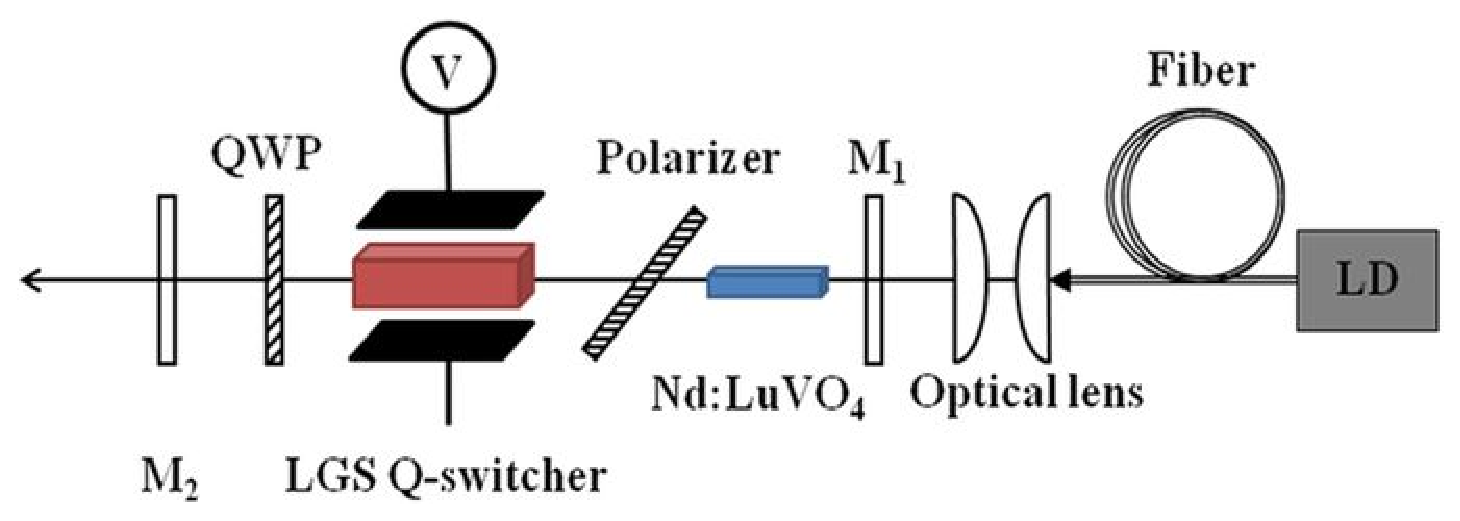
\includegraphics[height=3.25cm, width=1\linewidth]{act_q}} a) \\
\end{minipage}
\hfill
\begin{minipage}[h]{0.45\linewidth}
\center{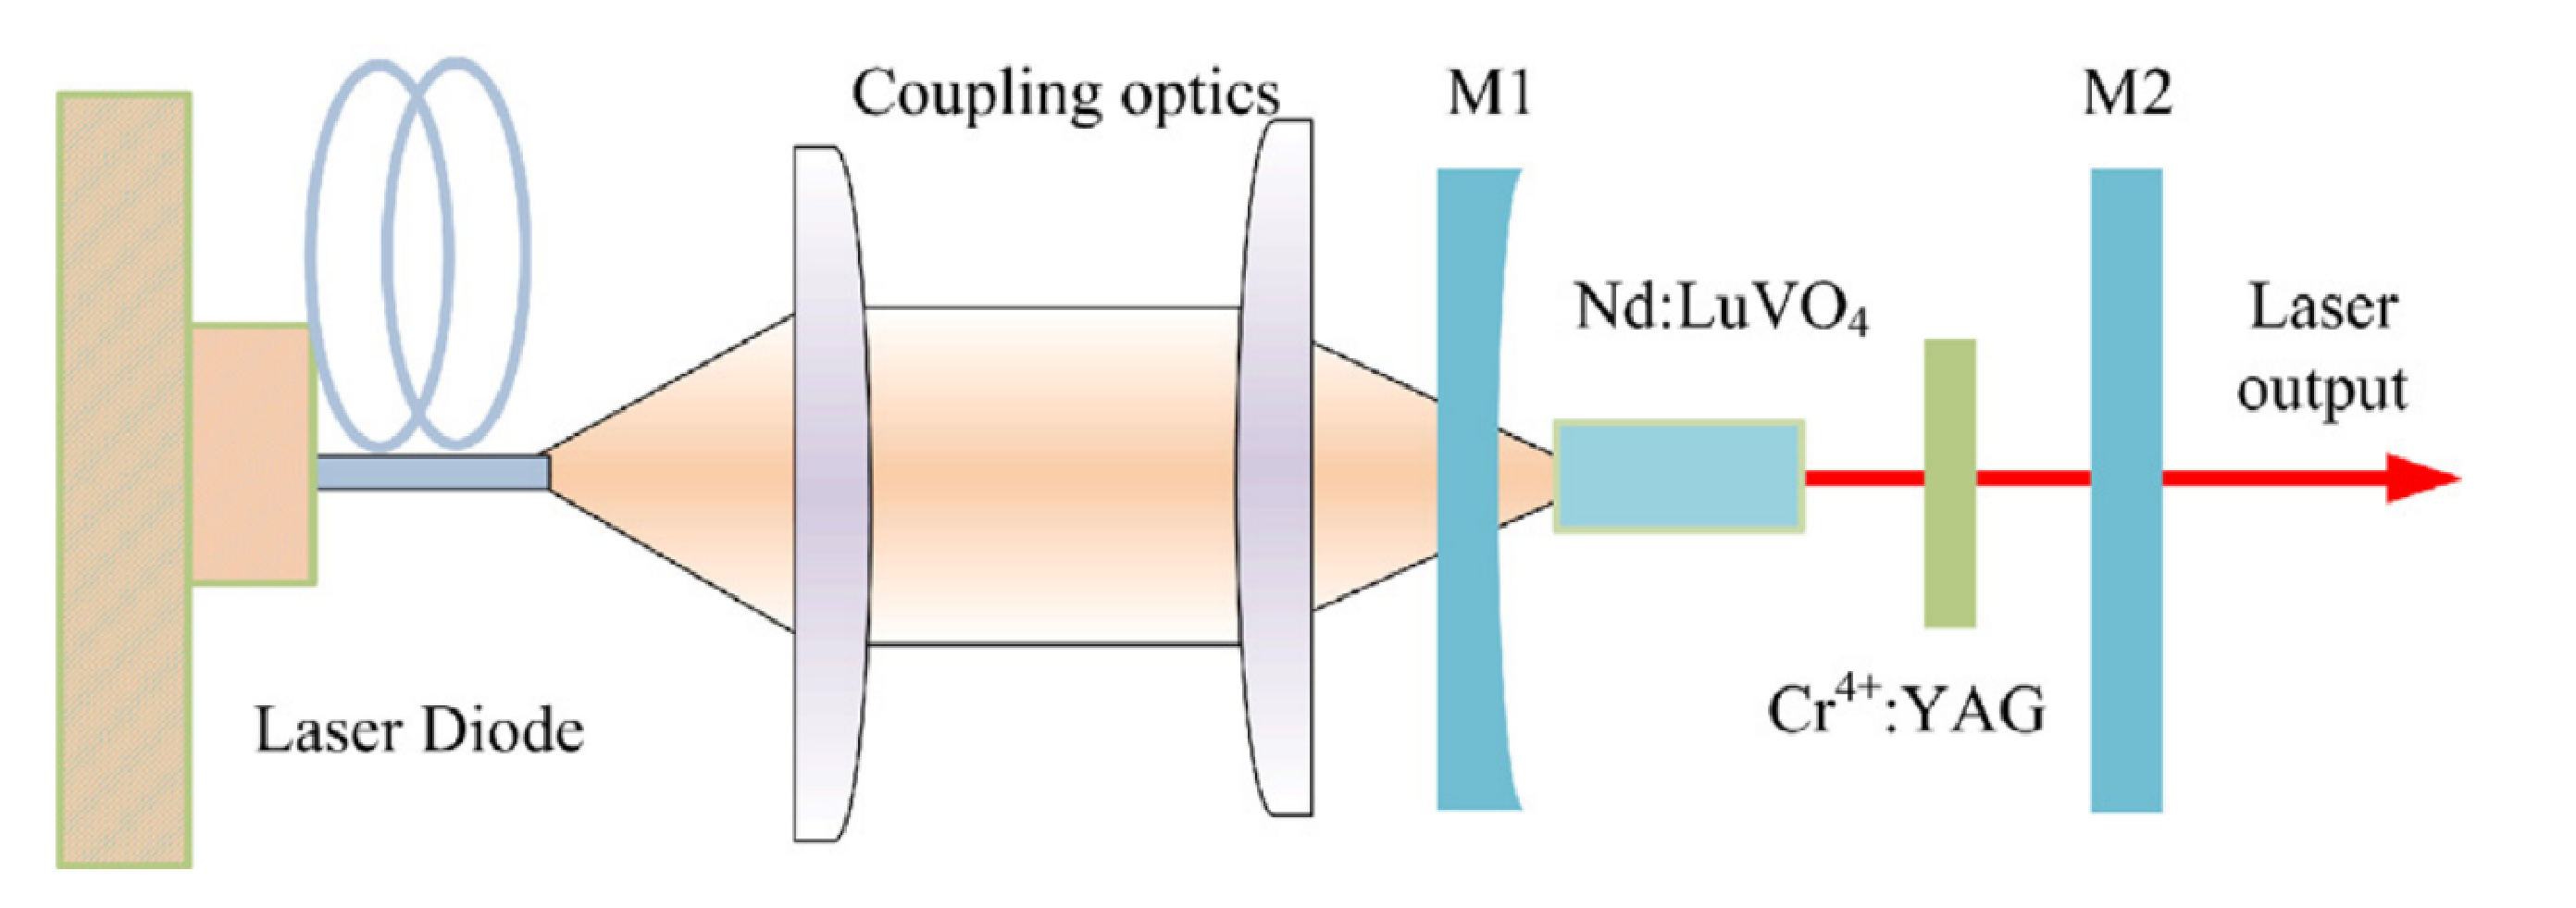
\includegraphics[height=3.05cm, width=1\linewidth]{pas_q}} \\b)
\end{minipage}


\caption{Typical Q-switched schemes for active and passive mode:
a) Laser diode end-pumped activelly Q-switched laser utilizing a langasite (LGS) crystal as an electro-optic Q-switch.
b) High repetition rate laser-diode end-pumped passively Q-Switched Nd:LuVO4/Cr4+:YAG
}
\label{fig:qs_lasers}
\end{figure}

In case of Q-switched lasers (Fig. ~\ref{fig:qs_lasers}), the pulse repetition rate is typically in the range from 1–100 kHz, sometimes higher. Passively Q-switched microchip lasers have reached pulse durations far below 1 ns and repetition rates up to several megahertz, whereas large (typically amplified) laser systems can deliver pulses with many kilojoules of energy and durations in the nanosecond range. For active Q-switching, the losses are modulated with an active control element (active Q-switch), typically either an acousto-optic or electro-optic modulator. Here, the pulse is formed shortly after an electrical trigger signal arrives. There are also mechanical Q-switches such as spinning mirrors, used as end mirrors of laser resonators. In any case, the achieved pulse energy and pulse duration depends on the energy stored in the gain medium, i.e. on the pump power and the pulse repetition rate.
For passive Q-switching (sometimes called self Q-switching), the losses are automatically modulated with a saturable absorber.
Here, the pulse is formed as soon as the energy stored in the gain medium (and thus the gain) has reached a sufficiently high level. In many cases, the pulse energy and duration are then fixed, and changes of the pump power only influence the pulse repetition rate.
Compared with active Q-switching, passive Q-switching is simple, takes up little space and cost-effective (eliminating the modulator and its electronics), and is suitable for very high pulse repetition rates. However, the pulse energies are typically lower. 
Unfortunatelly, closest for our wavelength interset are based on a neodymium-doped laser crystal which are applicable for Q-switching lay in the wavelength range $\sim$ 1 um, such as
Nd:YVO4/Cr4+:YAG 914 nm [1][2], Nd:GdVO4/Cr4+:YAG 912 nm [3][4], Nd:LuVO4/Cr4+:YAG 916 nm [5].
Due to the size of laser system, the best solution is passive Q-switched microchip laser: alignment-free monolithic solid-state laser where the laser crystal (or glass) is directly contacted with the end mirrors of the laser resonator (Fig. \ref{fig:micro}).

\begin{figure}[h]
\center{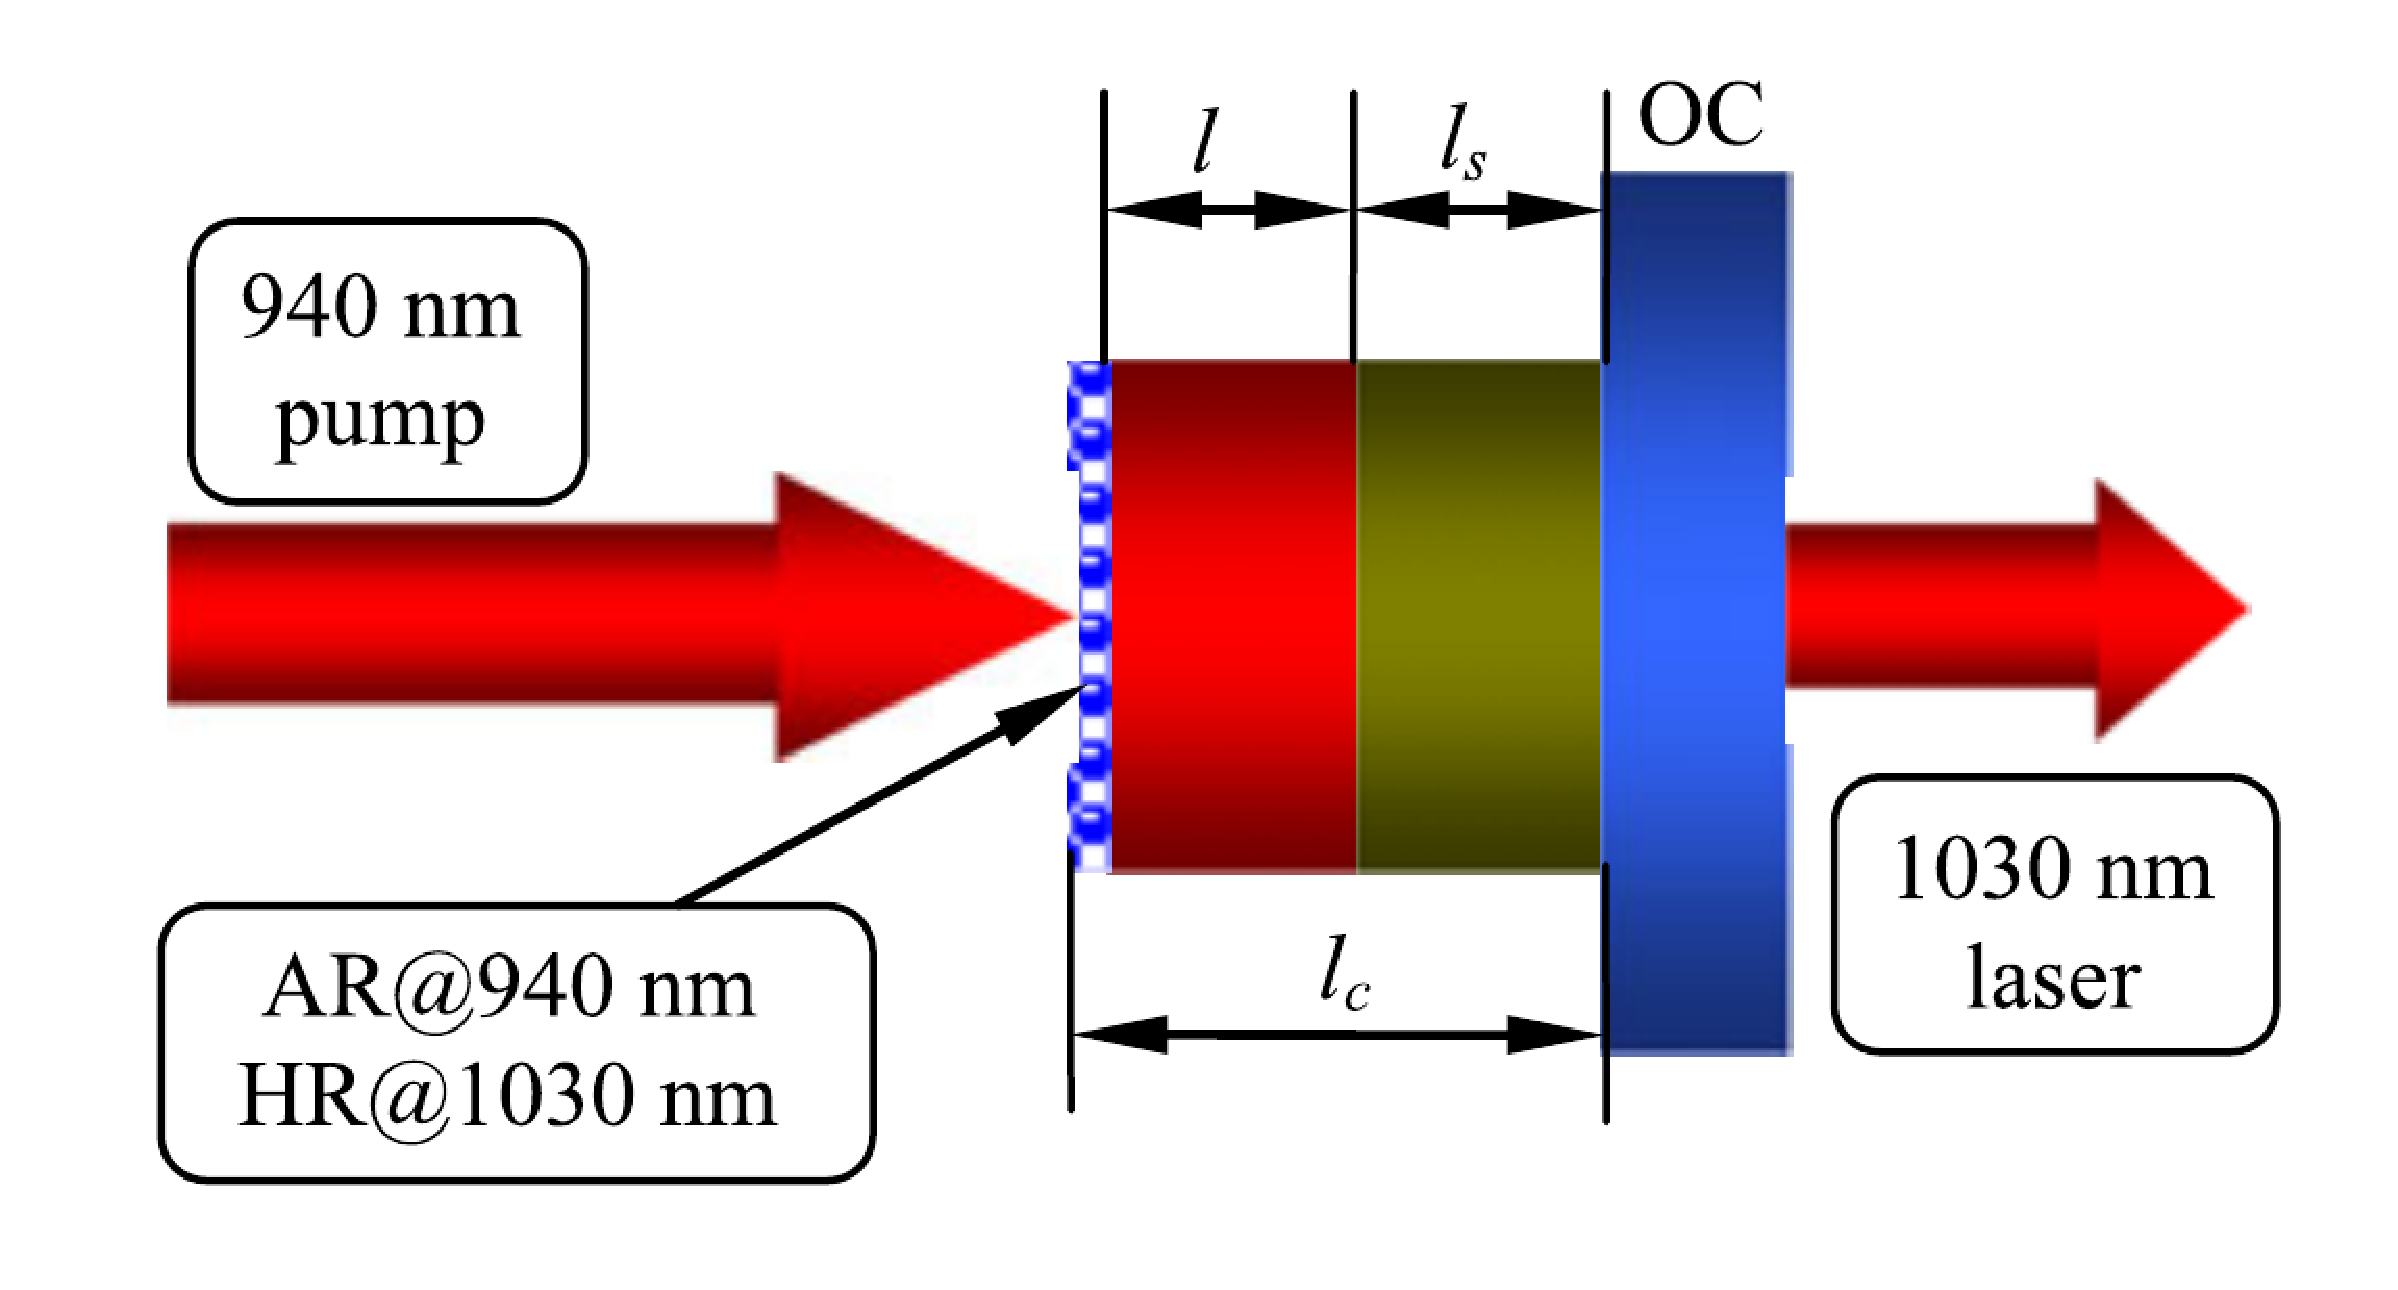
\includegraphics[width=0.55\linewidth]{micro}}
\vspace{1cm} 
\caption{The experimental setup of laser-diode pumped Yb:YAG/Cr:4+:YAG composite ceramics passively Q-switched laser. OC is the output coupler.}
\label{fig:micro} 
\end{figure}

Q-switched microchip lasers also allow the generation of unusually short pulses with durations below 1 ns, in extreme cases even below 100 ps. This holds particularly for passive Q switching with a SESAM [2], but it is also possible to use a saturable absorber crystal e.g. of Cr:YAG or some Cr-doped ceramics [1].

\subsubsection{The laser choice}
Eventually according to numerical simulation [1,2] the minimum pump power for high-repetition laser system, which is satistied our requrements is quite big > 6-8W this is just for start trigger lasing at 10kHz ( for Nd:YVO4/Cr4+ with best transmission parameters). This is because, optical-to-optical efficiencies – typically of the order of 5-20\%.
At the same time, electrical-to-optical efficiencies sometimes even above 60\%.

Therefore, we are trying to use a laser diode. Fortunately there is powerful high-repetition rate laser diode with quite short pulse duration $\sim 10ns$ at 905 nm from OSRAM Opto Semiconductors (Fig. \ref{fig:osram}).
Despite the fact that the amplification of the detector at this wavelength is small,
the laser power exceeds these losses, moreover at this wavelength the noise is smaller. 
Also it is eye-safe, that expand spectrum of possible applications.

\begin{figure}
\begin{floatrow}
\ffigbox{
\center{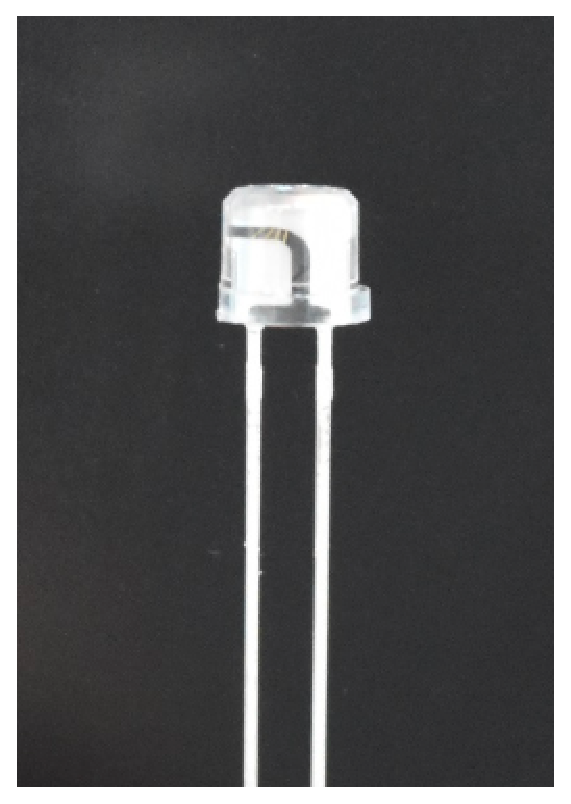
\includegraphics[width=0.45\linewidth]{osram}} 
}{
  \caption{Osram laser diode}%
\label{fig:osram} % or change caption location
}
\capbtabbox{

  \begin{tabular}{|M{4cm}|M{2.5cm}|}
\hline
Peak output power: & \textbf{75 $\pm$ 10 W}  \\ \hline
Forward current: & \textbf{40 A}  \\ \hline
Repetition rate: & \textbf{$\sim$ 100 kHz} \\\hline
Pulse duration: & \textbf{$\geq$ 10 ns} \\\hline
Emission wavelength, $\lambda$: & \textbf{905 $\pm$ 10 nm} \\\hline
Rise time: & \textbf{1 ns} \\  \hline
Fall time: & \textbf{1 ns} \\  \hline
Emmiting area: & \textbf{200 x 10 um} \\  \hline
Beam divergence: & \textbf{25$\pmb{{^\circ}}$ x 9$\pmb{{^\circ}}$} \\  \hline
Operating temperature: & \textbf{-40 .. 100 }$\pmb{{^\circ}}$\textbf{C} \\  \hline
\end{tabular}
}{%
\caption{OSRAM Laser diode characteristics}
\label{tbl:osram_datasheet}
}
\end{floatrow}
\end{figure}





%%%%%%%%%%%% LASER COLLIMATOR SUB-SECTION %%%%%%%%%%%
\subsection{Laser collimator}
\subsubsection{Analytical calculations}

Radiation characteristic of laser diode features carries due to its small size, light
quality, low threshold, low cost, these properties the laser diode play an important role in the information time, especially in the field of communication LIDAR.
Optical system is an essential part, which plays an important role in decreasing the divergence angle and homogenizing the beam spot which have an immense
influence on the light signal back from the target.
Together with the detector's collimator, a system with high resolution and high SNR can be obtained.
The design of the system was done by using ZEMAX model which also includes shaping and zooming features of design model.

\begin{figure}[H]
\begin{minipage}[h]{0.52\linewidth}
\center{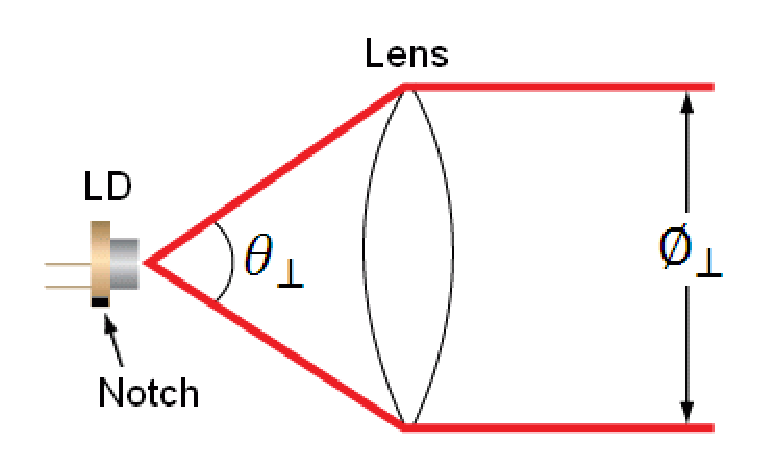
\includegraphics[height=3.15cm, width=0.85\linewidth]{laser_beam_3}} \\ a) 
\end{minipage}
\hfill
\begin{minipage}[h]{0.45\linewidth}
\center{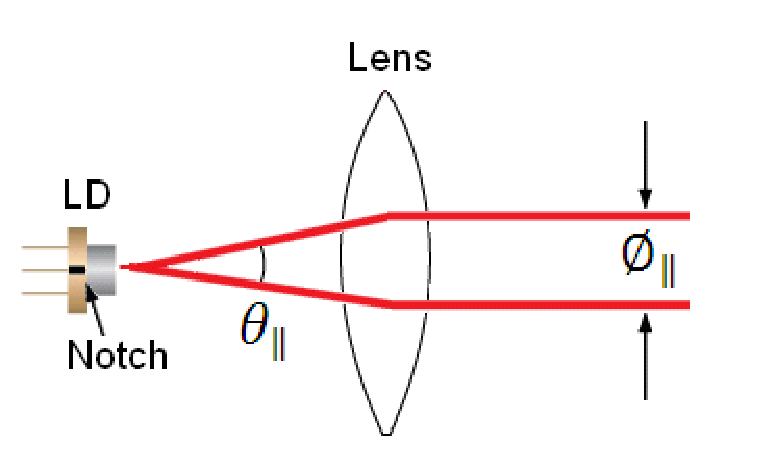
\includegraphics[height=3.25cm, width=1\linewidth]{laser_beam_4}} \\ b)
\end{minipage}
\caption{
In the above schematics, LD denotes the laser diode, \O$_{||}$ and \O$_{\perp}$ are the beam diameters in the parallel and perpendicular orientations, respectively, and $\theta_{||}$
 and  $\theta_{\perp}$ are the divergence angles in the parallel and perpendicular orientations, respectively.\\
a) Perpendicular beam divergence from laser diode.
b) Parallel beam divergence from laser diode.
}
\label{fig:laser_beam}
\end{figure}

The beam divergences of an edge-emitting laser diode will be different in the parallel and perpendicular directions, leading to an elliptical beam (Fig. \ref{fig:laser_beam}).
This can be compensated for by inserting anamorphic prism pairs or cylindrical lenses into the collimated beam, but in our case it's not needed.

Since the output of a laser diode is highly divergent, collimating optics are necessary. 
Traditional spherical lenses have a simple shape that can be
described as an arc of a circle and can be specified using
only a radius of curvature. Although these lenses are simple
to manufacture and inexpensive to use, they suffer in
performance due to a phenomenon called spherical
aberration. This inherent defect is due to the fact that a
spherical shape is not the ideal shape for a focusing or
collimating lens to be. The ideal case is a more complex
shape that is typically defined using a radius of curvature, a
parabolic term (conic), and several high order coefficients.
The complex shape of aspheric lenses allows for correction
of spherical aberration. This provides better quality
collimated beams for collimating applications, a smaller spot
size for focusing applications, and better image quality for
imaging applications. In fact, in many cases just a single
aspheric lens can take the place of several conventional
spherical lenses, leading to a lighter, more compact, less
expensive, and better performing optical system. Aspheres
are now a viable design option for many applications.
Choosing an appropriate aspheric lens for collimating a laser diode is essential, as the resulting beam size and transmission range are dependent on the lens used.

To calculate the beam size of a collimated laser diode, we first need to know its divergences and area of emitting surface.
The specifications for the OSRAM laser diode indicate that the perpendicular and parallel beam divergences are 25${^\circ}$ and 9${^\circ}$, respectively. Because of this asymmetry in the two axes, an elliptical beam will form as the light diverges. To collect as much light as possible during the collimation process, consider the larger of these two divergence angles in any calculations (i.e. 25${^\circ}$).

In paraxial approximation, for beam diameter calculation after passing lens  the following formula is using (Fig. \ref{fig:laser_beam}):

\begin{equation}\label{eq:beam_size}
\text{\O}_{\perp} = 2 \cdot f \cdot \tan{(\frac{\theta_{\perp}}{2})}
\end{equation}

For beam divergence after passing the optical system (Fig. \ref{fig:lens}):



\begin{figure}[H]
\begin{minipage}[h]{0.52\linewidth}
\center{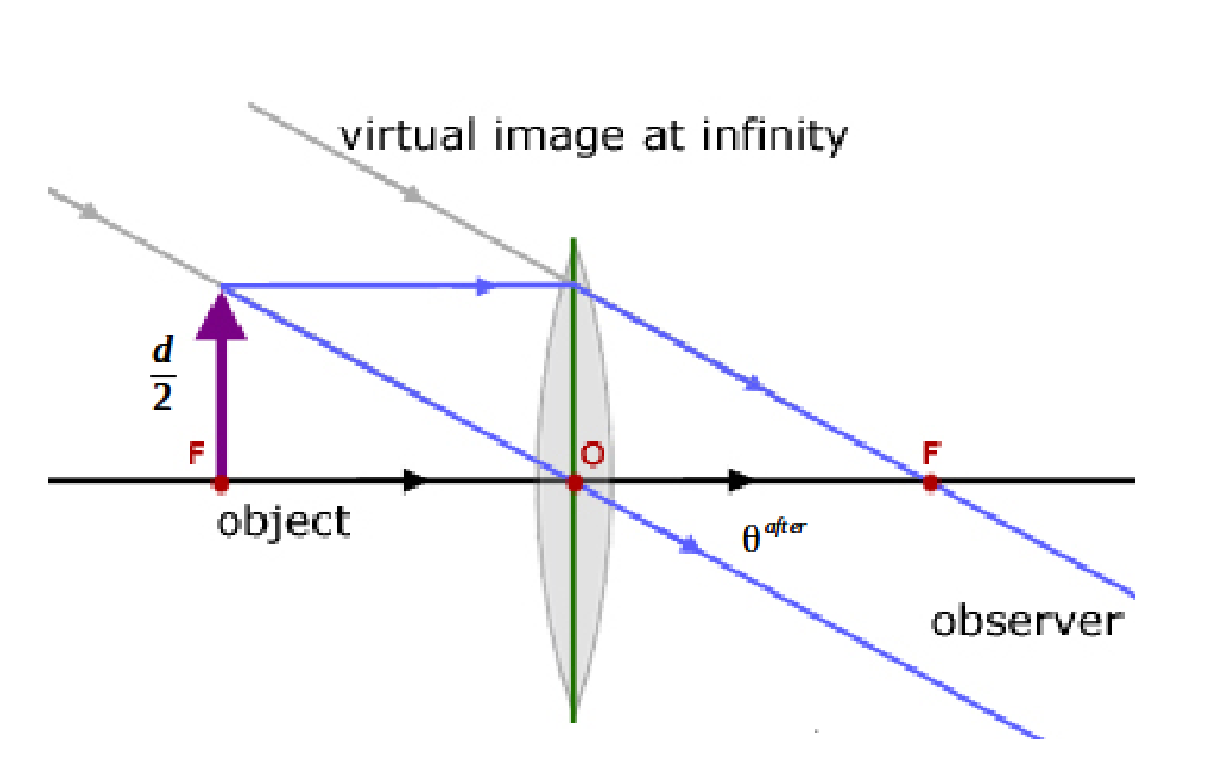
\includegraphics[width=1.2\linewidth]{lens}}
\end{minipage}
\hfill
\begin{minipage}[h]{0.45\linewidth}
\begin{equation}\label{eq:beam_divergence}
\theta^{after} = 2 \cdot \tan^{-1}{(\frac{d}{2f})}
\end{equation}
\end{minipage}
\caption{
Simple demonstration, shows divergence of the beam emitted from object, seated at the focus of the optical system. Here, d is the size of emitting area of laser diode (200 um in our case), f is total focal length of the optical system.
}
\label{fig:lens}
\end{figure}





From the formulas \ref{eq:beam_size} \ref{eq:beam_divergence}, it is obvious that the larger the focal lens, the larger the diameter of the beam and the smaller the beam divergence. It means, that by increasing focal length we can achieve the desirable level of divergence (up to diffraction limit, with assumption we free of aberrations). But, by increasing focal length the beam diameter is also increased.
Since the size of MEMS is only 3.5 mm, we have limitation for focal length (we want reflect all light which are emitted).
The same result can be getting from the Lagrange invariant relationship between the heights and angles of any two rays propagating through the system (in case of linearity of paraxial optics).

Important to note, that even a well-collimated beam has a non-vanishing divergence because of wave-nature of the light, the beam diameter varies (for large distances) with the distance from the laser diode collimator. The resulting beam divergences of the collimated beam:



\begin{equation}\label{eq:beam_divergence}
\theta_{\perp/||} = \frac{2\cdot \lambda}{\pi \cdot \text{\O}_{\perp/||}}
\end{equation}

% \newpage
\subsubsection{The optical system choice}
According to formula \ref{eq:beam_size}, our focal length should be $\sim$ 6.5 mm.
The first way is just using nearest suitable aspherical lens, which has focal length 6.2 mm (Fig. \ref{fig:ld_lens}).
These laser molded aspheric lense fulfilled all our the needs. Also, this aspheric lens is anti-reflection coated for optimum transmission in the 600 - 1050 nm wavelength range. The anti-reflection coating provides <0.4\% average reflection over the entire design wavelength range. By utilizing a single aspheric lens, the need for a multi-lens system is eliminated, allowing for a more compact and robust design. 


\begin{figure}
\begin{floatrow}
\ffigbox{
\center{
\includegraphics[width=0.65\linewidth]{ld_lens}} 
}{
  \caption{Aspheric lens used for laser collimator}%
\label{fig:ld_lens} % or change caption location
}
\capbtabbox{

  \begin{tabular}{|M{4cm}|M{4cm}|}
\hline
Effective Focal length: & \textbf{6.2 mm} \\  \hline
Clear Aperture: & \textbf{3.7 mm} \\  \hline
Numerial aperture (NA): & \textbf{0.3} \\  \hline
Material: & \textbf{D-ZK3}  \\ \hline
Center Thickness: & \textbf{3.484 mm}  \\ \hline
Coating: & \textbf{ BBAR (600 - 1050 nm)} \\  \hline
\end{tabular}
}{%
\caption{Aspheric lens characteristics}
\label{tbl:ld_lens_datasheet}
}
\end{floatrow}
\end{figure}



The second way is using two cylindrical lenses for each axis separately (Fig. \ref{fig:cylindrical_lens}). 
This allows the use of a lens with a large focal length, because the divergence of the parallel axis is 9$^\circ$, not 25$^\circ$.


\begin{figure}
\begin{floatrow}
\ffigbox{
\center{
\includegraphics[width=0.65\linewidth]{cylinder_lens}} 
}{
  \caption{Two cylindrical lens used for laser collimator}%
\label{fig:cylindrical_lens} % or change caption location
}
\capbtabbox{

  \begin{tabular}{|M{3.5cm}|M{2cm}|M{2cm}|}
\hline
Effective Focal length: & \textbf{8 mm} & \textbf{12 mm} \\  \hline
Clear Aperture: & \textbf{4 mm} & \textbf{5.4 mm}\\  \hline
Numerial aperture (NA): & \textbf{0.31} & \textbf{0.25}\\  \hline
Material: & \textbf{N-BK7}  & \textbf{N-BK7}\\ \hline
Center Thickness: & \textbf{3 mm}  & \textbf{2.2 mm}\\ \hline
Coating: & \textbf{ BBAR (600 - 1050 nm)} & \textbf{12 mm} \\  \hline
\end{tabular}
}{%
\caption{Two cylindrical lens characteristics (for each axis)}
\label{tbl:ld_cylinder_lens_datasheet}
}
\end{floatrow}
\end{figure}



\subsubsection{ZEMAX simulation}

Once the analytical calculations are completed, and the system variables are determined, the ZEMAX optical design program is used to simulate a specific example.
ZEMAX is a design software containing features and tools to design, optimize, and analyze any optical system.



\begin{figure}[H]
\begin{minipage}[h]{0.48\linewidth}
\center{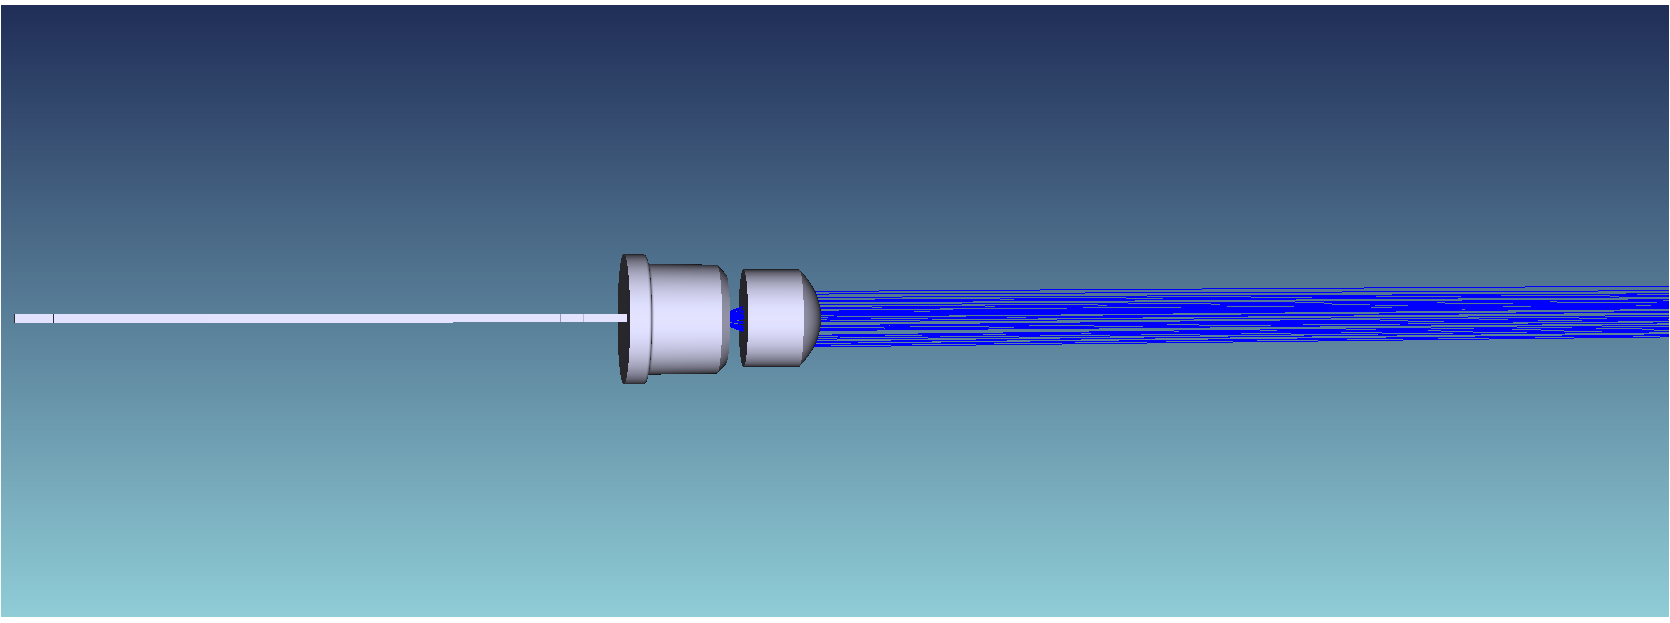
\includegraphics[height=3.25cm, width=1\linewidth]{zem_1_lens}}\\ a)
\end{minipage}
\hfill
\begin{minipage}[h]{0.45\linewidth}
\center{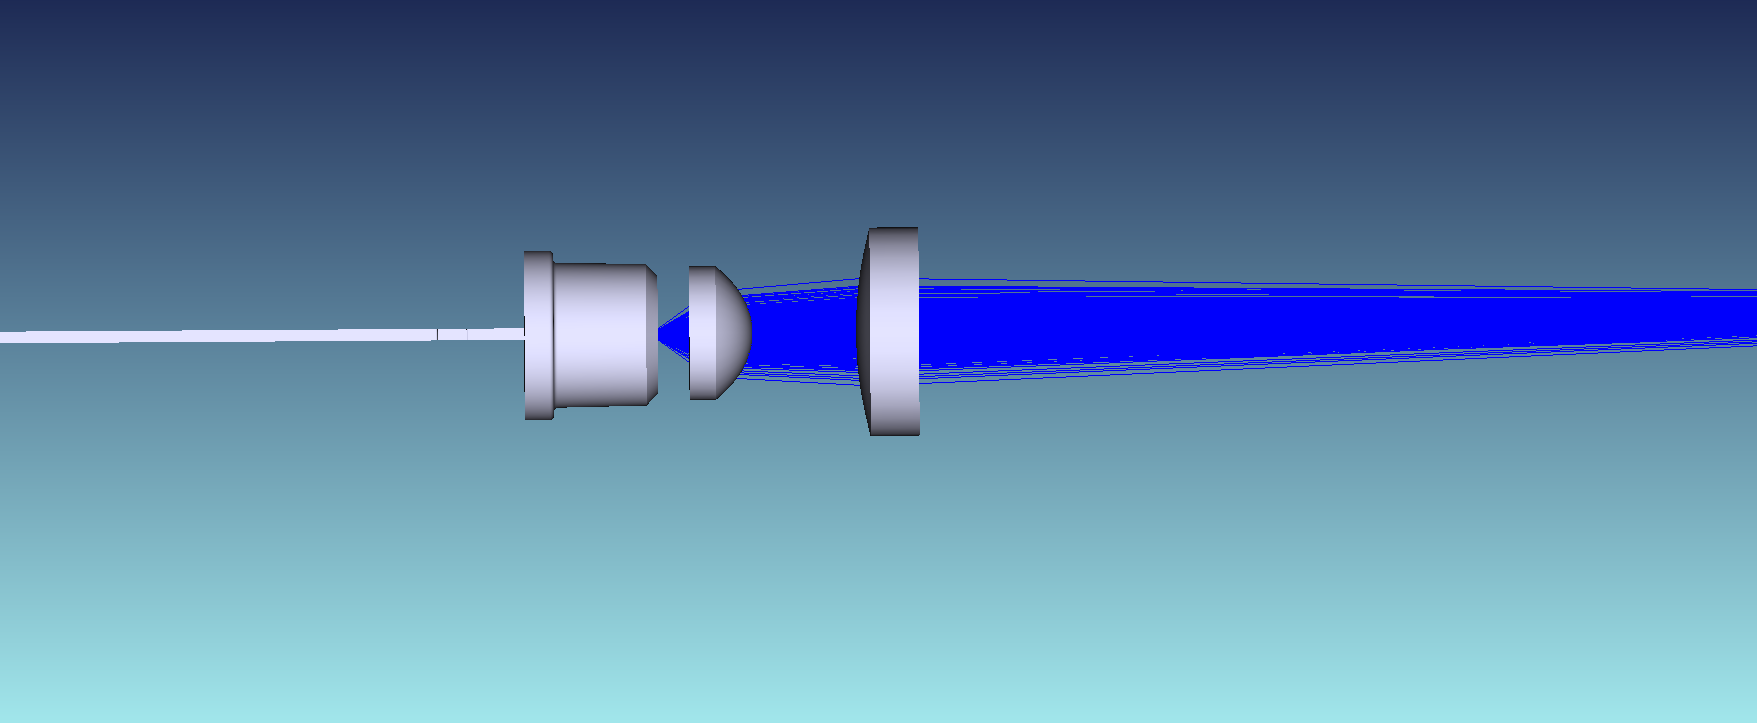
\includegraphics[height=3.25cm, width=1\linewidth]{zem_2_lens}}\\ b)
\end{minipage}
\vfill
\begin{minipage}[h]{0.495\linewidth}
\center{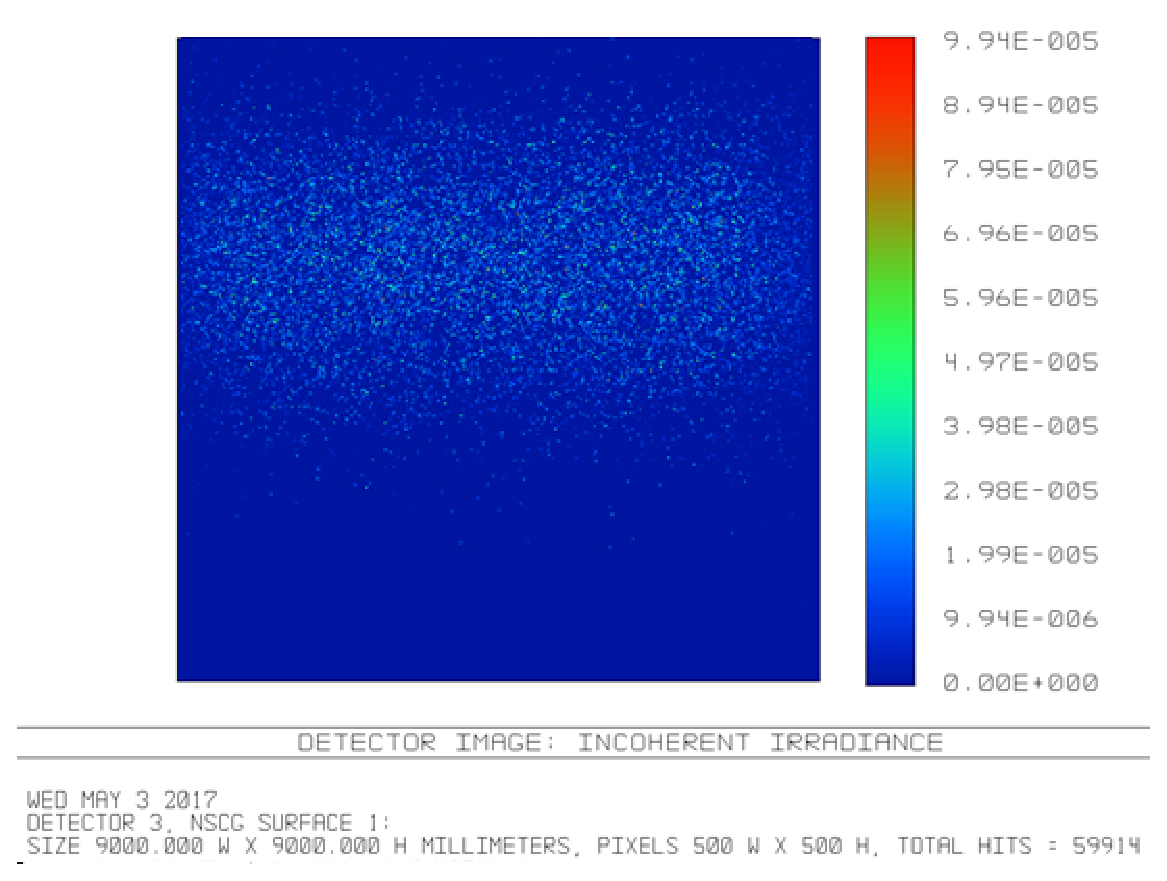
\includegraphics[height=6cm, width=1\linewidth]{spot_1_lens}} \\ c)
\end{minipage}
\hfill
\begin{minipage}[h]{0.495\linewidth}
\center{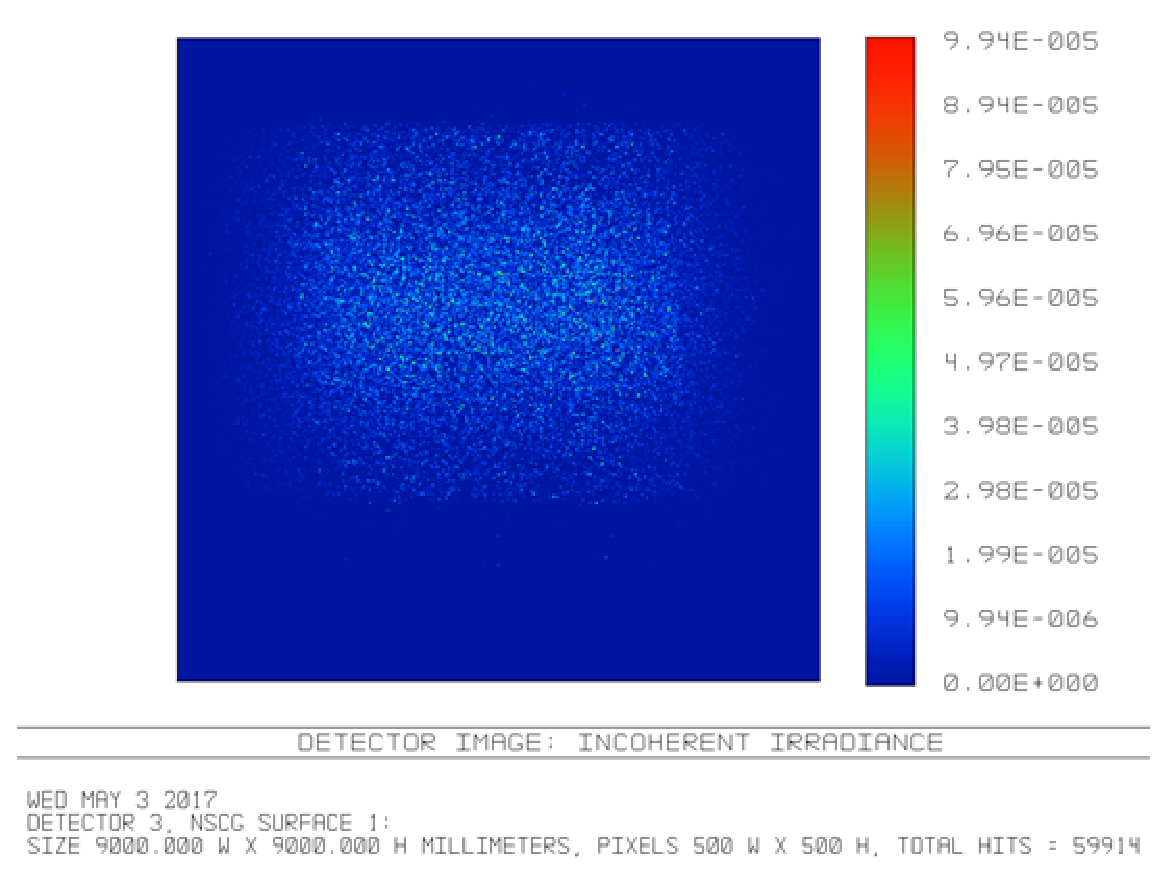
\includegraphics[height=6cm, width=1\linewidth]{spot_2_lens}} \\ d)
\end{minipage}

\caption{The ray tracing and  also beam spots results are obtained using non-sequential Zemax mode, the laser diode was simulated based on real ray-data file (5M rays) from OSRAM site.
a) The ray traycing for sinle-lens collimator.
b) The ray traycing for two-lens collimator.
c) Spot diagram for sinle-lens collimator.
d) Spot diagram for two-lens collimator.
}
\label{fig:spot_simulation}
\end{figure}





The ray tracing results obtained using ZEMAX are presented in (Fig. \ref{fig:spot_simulation}.a)) for the single-lens system and in (Fig. \ref{fig:spot_simulation}.b)) for the two-lens system.
Beam spots obtained with ZEMAX are presented in (Fig. \ref{fig:spot_simulation}.c)) and (Fig. \ref{fig:spot_simulation}.d)) for the single-lens and two-lens systems, respectively. 
As can be seen, in the case of a system of two lenses, the beam has a smaller divergence, as expected.
But, a first design method seems to be more practical than the second one, since there is only
one lens, and it might be easier to align a single-lens system than to align a two-lens system.
However, the two-lens system has more degrees of freedom, and therefore, the optical
parameters can be more widely adjusted.
Also considering the size of it, it may get bulky and hard to use.
Therefore, as a compact collimator a single-lens collimator used, whose length is 10 mm, and diameter 6 mm.



The simulation results verify the availability that the beam from the laser diode meets the requirements after optical emission from system.
Simulation was also made in a sequential mode just in case (Fig. \ref{fig:ld_sequential}).


\begin{figure}[h]
\center{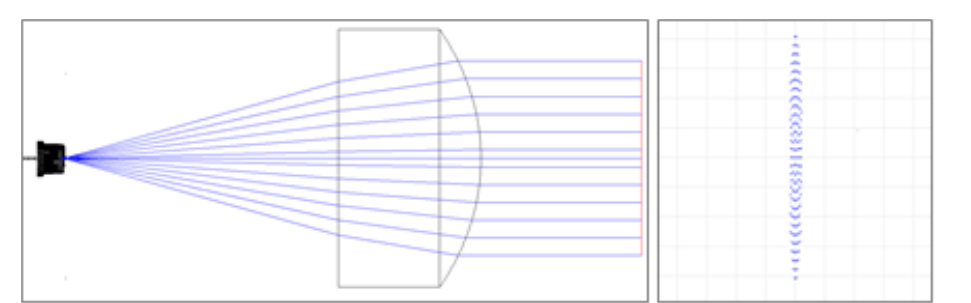
\includegraphics[width=1\linewidth]{ld_sequential}}
\caption{Ray-traycing of single-lens collimator based on aspheric lens in sequential mode}
\label{fig:ld_sequential} 
\end{figure}

\subsubsection{Assembled laser collimator}
As a result, the assembled compact laser collimator with an integrated OSRAM diode is shown in the Fig. \ref{fig:ld_assembled}.
This colimator provide beam angular size is 0.1$^\circ$ x 2.5$^\circ$, by having length only 10 mm, and diameter 6 mm.

\begin{figure}[h]
\center{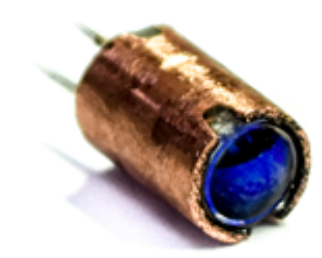
\includegraphics[width=0.2\linewidth]{ld}}
\caption{Assembled compact laser collimator}
\label{fig:ld_assembled} 
\end{figure}



%%%% LASER DRIVER SECTION %%%%
\subsection{Laser driver}
% \noindent

% \vfill
% \begin{minipage}{1\textwidth}
% \center{
% \includegraphics[width=1\linewidth]{our_laser_driver}
% }
% \caption{Assembled compact laser collimator}
% \label{fig:ld_assembled} 
% \end{minipage}
% \hfill
% \begin{minipage}{0.4\textwidth}

To operate Osram laser diode the laser driver is required.
The LDP-AV 40-70 is the smallest available source for nanosecond pulses (Fig \ref{fig:laser_driver}).
It provides 40A with fixed pulse duration of 5 ns at repetition rate up to 100kHz.

% \begin{minipage}{1\textwidth}
\begin{figure}[H]
\center{
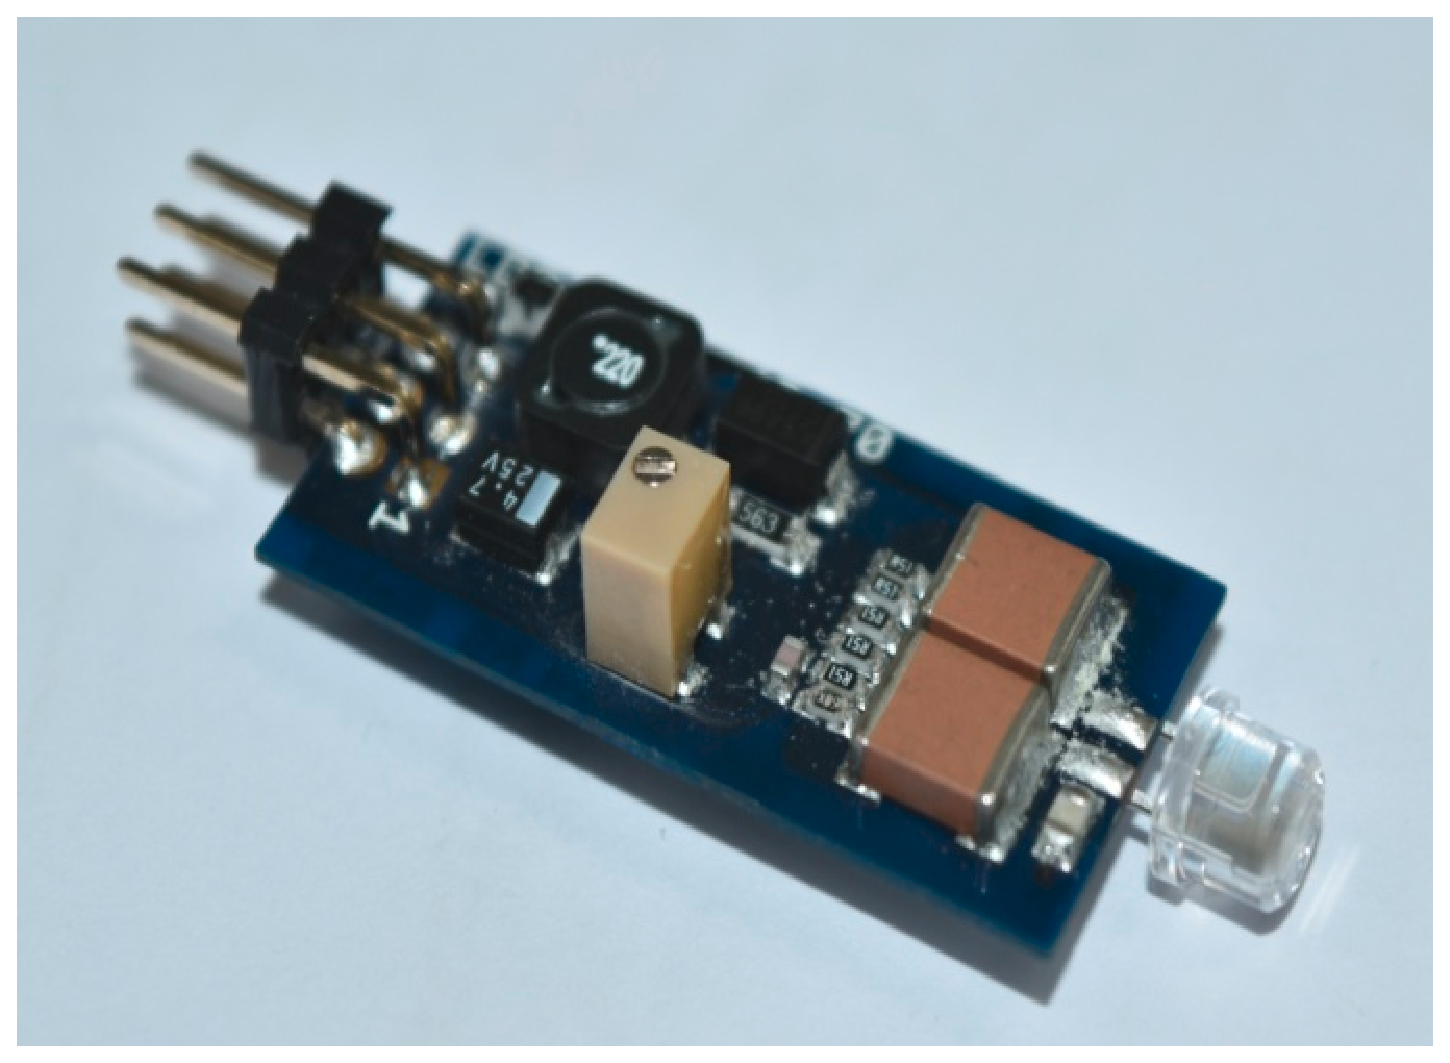
\includegraphics[width=0.4\linewidth]{laser_driver}
\caption{Commercial laser driver with attached Osram diode.}
\label{fig:laser_driver}
}
\end{figure}

 % Bottom one is output of detector catched by 2GSa/s oscilloscope after laser shoot. 

% \hfill
% \includegraphics[width=0.45\linewidth]{laser_output}
% } 
% \vspace{-3mm}
% \end{minipage}

% \end{minipage}

Our team made an analog of this laser driver, smaller in size with the same characteristics. The device optimized for size and functionality (Fig. \ref{fig:our_laser_driver}).

Figure \ref{fig:laser_output} shows the screenshot of the 2Gsa/s oscilloscope, as can be seen, the pulse duration is of the order of 10 ns. The detector was SiPM which is described in the next section.

\begin{figure}
\begin{floatrow}
\ffigbox{
\center{\includegraphics[width=0.45\linewidth]{our_laser_driver}} 
}{
  \caption{Our laser driver.}%
\label{fig:our_laser_driver} % or change caption location
}
\ffigbox{
\center{\includegraphics[height=6cm, width=1\linewidth]{laser_output}} 
}{
  \caption{Output of detector catched by 2GSa/s oscilloscope after laser shoot.}%
\label{fig:laser_output} % or change caption location
}
\end{floatrow}
\end{figure}






\subsection{Completed laser module}

Finally we got laser system with the following params:

\begin{table}[H]
\label{tbl:rfp_laser}
\begin{center}
\begin{tabular}{|p{0.2\linewidth}|p{0.3\linewidth}|}
\hline
Pulse energy: & \textbf{$\sim$ 1 uJ}  \\ \hline
Repetition rate: & \textbf{12 kHz} \\\hline
Pulse duration: & \textbf{$\leq$ 10 ns} \\\hline
Wavelength, $\lambda$: & \textbf{905 nm} \\\hline
Power consumption: & \textbf{$\leq$ 0.25 W} \\  \hline
Dimension: & \textbf{$\leq$ 3 cm$^3$} \\  \hline
\end{tabular}
\caption{Characteristics of the laser system}
\end{center}
\end{table}


The repetition rate is tunable parameter, it was chosen in consideration of low power consumption and obtaining a good enough pixels resolution.


\section{MEMS module}

\section{SiPM module}
\subsection{SiPM detector}
The Silicon Photomultiplier (SiPM) is a single-photon sensitive sensor that has
performance characteristics comparable to a conventional ICCD/PMT/APD (Table ~\ref{tbl:sipm_comparison}).
with the practical advantages of a solid-state sensor. 


\begin{figure}[H]
\begin{center}
\begin{tabular}{ |c|c|c|c|c| } 
\hline
& ICCD & PMT & APD & SiPM  \\
\hline
Sensitivity & $\sim 10$ ph.e & 1 ph.e & $\sim 10$ ph.e & 1 ph.e  \\ 
\hline
Gain & $10^3-10^6$ & $10^6$ & 100-200 & $10^6$ \\ 
\hline
Dynamic Range & large & $\sim 10^3$  & lasrge & $\sim 10^3/mm^2$\\ 
\hline
Operating Voltage & $\sim 100 V$ & 1-2 kV & 100-500 V & 20-50 V\\ 
\hline
Efficiency at blue & 50\% & 20\% & 50\% & 30\% \\ 
\hline
Timing & $\sim 1 ms$ & $\sim 100 ps$ & $\sim ns$ & $\sim 30 ps$\\ 
\hline
\end{tabular}
\vspace{-5mm}
\caption{Specification of the LIDAR scanning system}
\label{tbl:sipm_comparison}
\end{center}
\end{figure}


It is formed of a summed array of closely-packed Single Photon Avalanche Photodiode (SPAD) sensors (Fig. \ref{fig:sipm_structure})

\begin{figure}[H]
\center{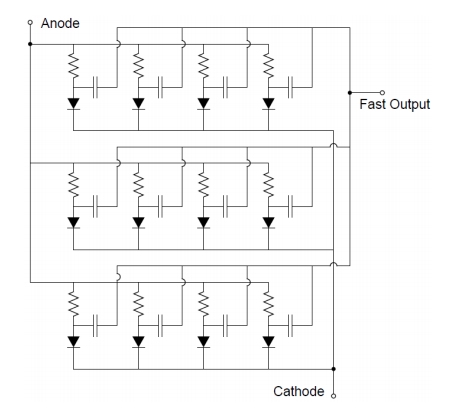
\includegraphics[width=0.5\linewidth]{sipm_structure}}
\caption{An SiPM consists of an array of microcells
(SPAD plus quench resistor) with summed output.}
\label{fig:sipm_structure}
\end{figure}


The SiPM is operated in Geiger-mode which enables high gain
(1x106), high detection efficiency (>50\%) and fast timing
(sub-ns rise times) at moderate bias (~30V). This is achieved by creating a high
field region in the diode that generates a self-perpetuating charge
avalanche when a photon is absorbed. Passive
quenching, is achieved through the use of a
series resistor which limits the current drawn by the diode during
breakdown. This lowers the reverse voltage seen by the diode to a
value below its breakdown voltage, thus halting the avalanche. The
diode then recharges back to the bias voltage, and is available to
detect subsequent photons.


Since the capacitance of the microcell will depend upon its area, the reset time will vary for different microcell sizes, with a 50mm
microcell SiPM having a significantly longer reset time and gain than a 10mm microcell SiPM.
Another one of the most important parameter is PDE (Photon Detection Efficiency). This is the product of the $QE\cdot AIP \cdot FF$, where $QE$ is quantum efficiency, $AIP$ is the avalanche initiation probability and $FF$ is the fill factor of the microcells.
The characteristics and PDE graph of the selected SiPM detector by Sensl are shown in the table \ref{tbl:sipm_characteristics} and figure \ref{fig:sipm_pde} correspondingly.


\begin{figure}[H]
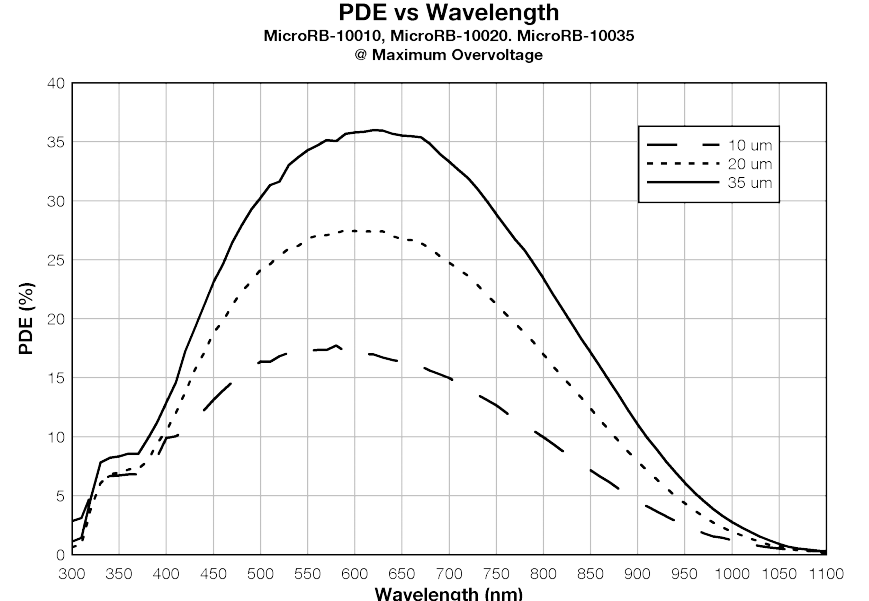
\includegraphics[width=1\linewidth]{sipm_pde}
\caption{PDE for different cell sizes.}
\label{fig:sipm_pde}
\end{figure}

\begin{table}[H]
\label{tbl:rfp_laser}
\begin{center}

\begin{tabular}{|p{0.2\linewidth}|p{0.3\linewidth}|}
\hline
Microsell size: & \textbf{$\pmb{35\; um}$}  \\ \hline
Gain: & \textbf{$\pmb{1.7 \cdot 10^6}$}  \\ \hline
PDE @ 905 nm: & \textbf{$\leq$ 10\%} \\\hline
Dark current rate: & \textbf{3.8 MHz} \\\hline
Dark current: & \textbf{1.5 uA} \\\hline
Rise time: & \textbf{3.7 ns} \\\hline
Recharge time: & \textbf{73 ns} \\  \hline
\end{tabular}
\vspace{-5mm}
\caption{Characteristics of the SiPM}
\label{tbl:sipm_characteristics}
\end{center}
\end{table}



In accordance with the characteristics of the detector, we can say that it is ideally suited for the LiDAR based on TOF technology. High gain and small rise time allows sigle-detection mode with high SNR, while small recharge time allow very high repetition rate, up to 10MHz.

Figure \ref{fig:sipm_pde} shows the SiPM experimental setup (left) and screenshot of the SiPM output after laser shooting (right), caught by the 2Gsa/s oscilloscope.


\begin{figure}[H]
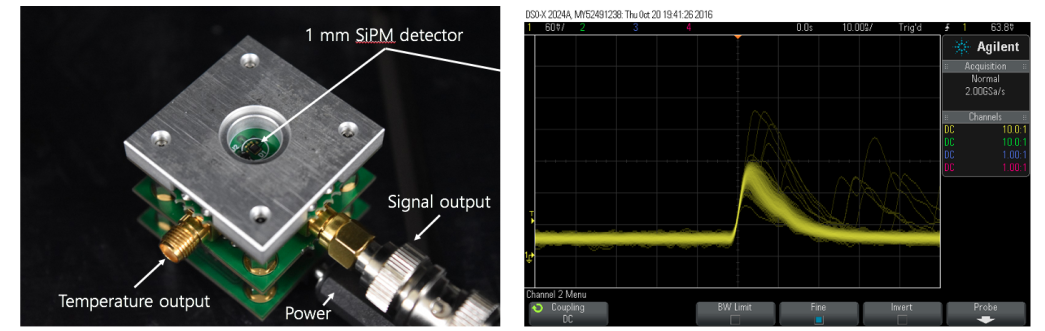
\includegraphics[width=1.05\linewidth]{sipm}
\caption{SiPM experimental setup (left) and output of SiPM after laser shooting (rigth).}
\label{fig:sipm_pde}
\end{figure}



\subsection{SiPM collimator}
Receiver optics is one of the most important in the whole system. It provides a specified FOV, minimizing noise. Our receiver aperture is limited by diameter of the MEMS, so it should not exceed 3.6mm.
Since we don't need wide FOV we are not suffering so much due to abberrations, thus the optical system consists of one aspherical lens to focus received signal to SiPM and a pinhole for cutting FOV according to eq:\ref{eq:sipm_FOV}.
FOV of SiPM should be big enough to cover laser beam, but at the same time should be quite small to decrease noise impact.


\begin{equation}\label{eq:sipm_FOV}
FOV = 2\cdot tan^{-1}(\frac{d}{2\cdot f})
\end{equation}
Where d is pinhole size, f is focal length.



\begin{figure}[h]
\begin{floatrow}
\ffigbox{
\center{
\includegraphics[width=0.65\linewidth]{ld_lens}} 
}{
  \caption{Aspheric lens used for SiPM collimator.}%
\label{fig:ld_lens} % or change caption location
}
\capbtabbox{

  \begin{tabular}{|M{4cm}|M{4cm}|}
\hline
Pinhole size: & \textbf{200 um} \\  \hline
Effective Focal length: & \textbf{4.5 mm} \\  \hline
Clear Aperture: & \textbf{3.7 mm} \\  \hline
Numerial aperture (NA): & \textbf{0.3} \\  \hline
Material: & \textbf{D-ZK3}  \\ \hline
Center Thickness: & \textbf{3.484 mm}  \\ \hline
Coating: & \textbf{ BBAR (600 - 1050 nm)} \\  \hline
\end{tabular}
}{%
\caption{Characteristics of optics for SiPM, bandpass filter should be improoved.}
\label{tbl:sipm_datasheet}
}
\end{floatrow}
\end{figure}


\begin{figure}[H]
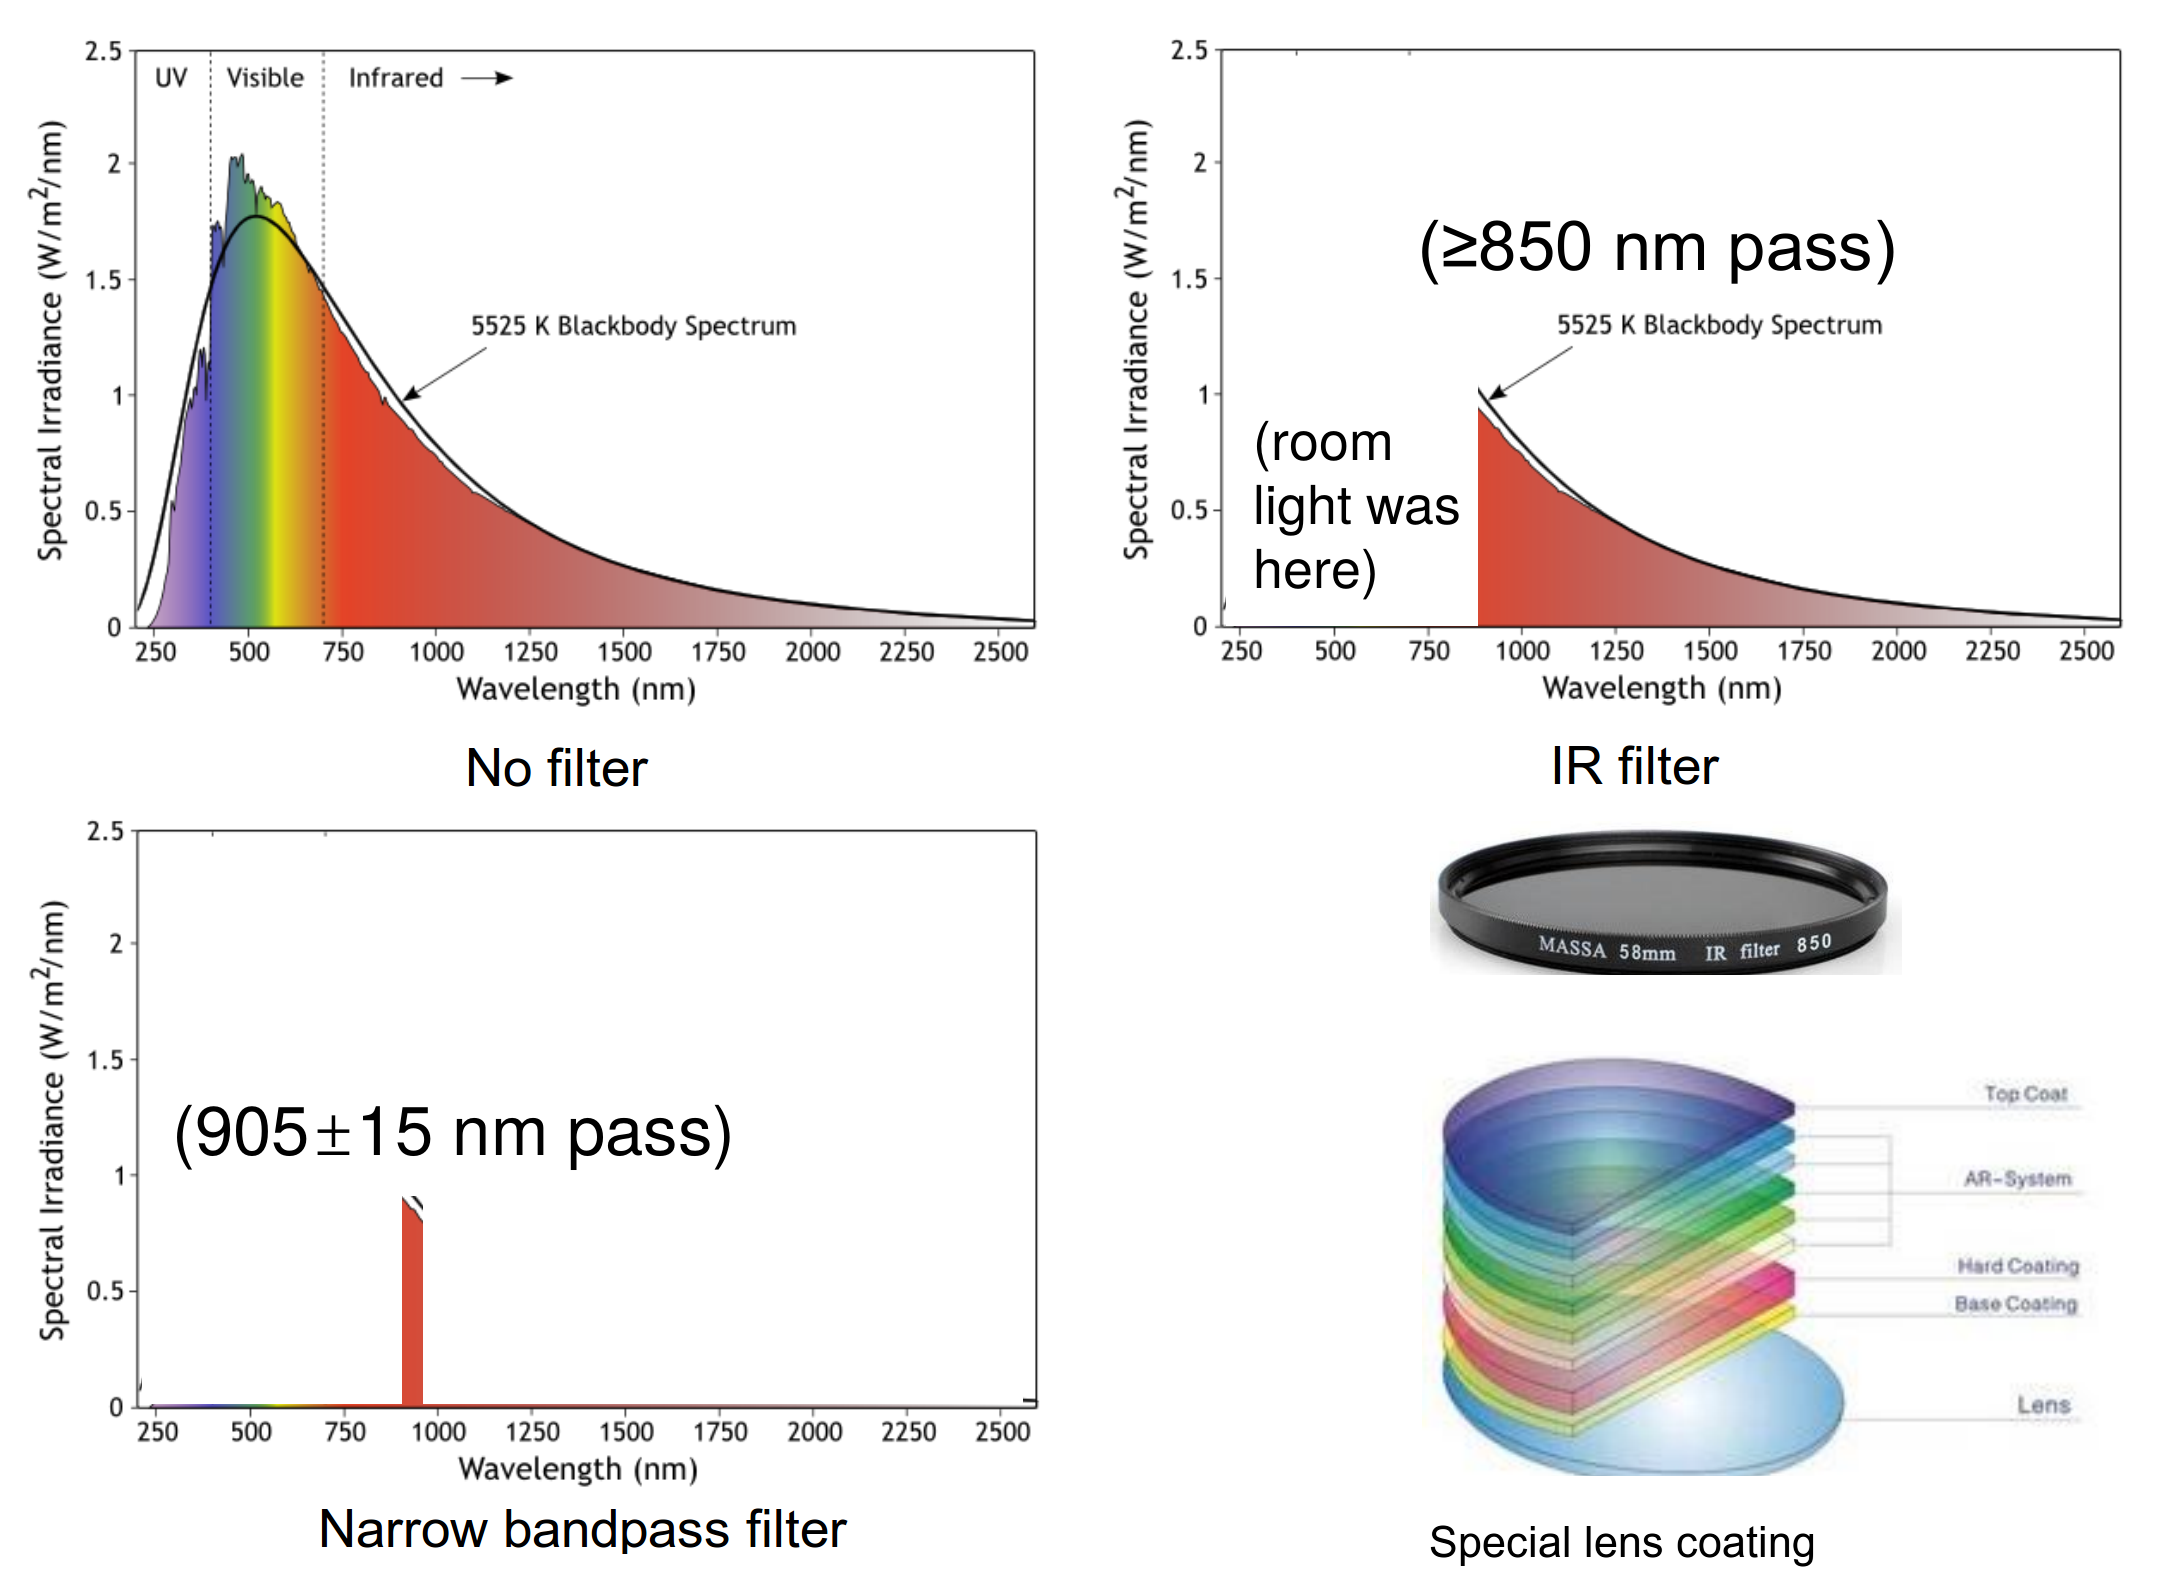
\includegraphics[width=1\linewidth]{coating}
\caption{Effect of the filter on the sun spectrum.}
\label{fig:coating}
\end{figure}

To make lidar could work in the daytime we should remove background as mush as we can, so an IR optical filter was built into the detector collimator. For sunny day the bandpass filter with 10nm bandwidth should be implemented, i.e by lens coating (Fig. \ref{fig:coating})



\begin{figure}[H]
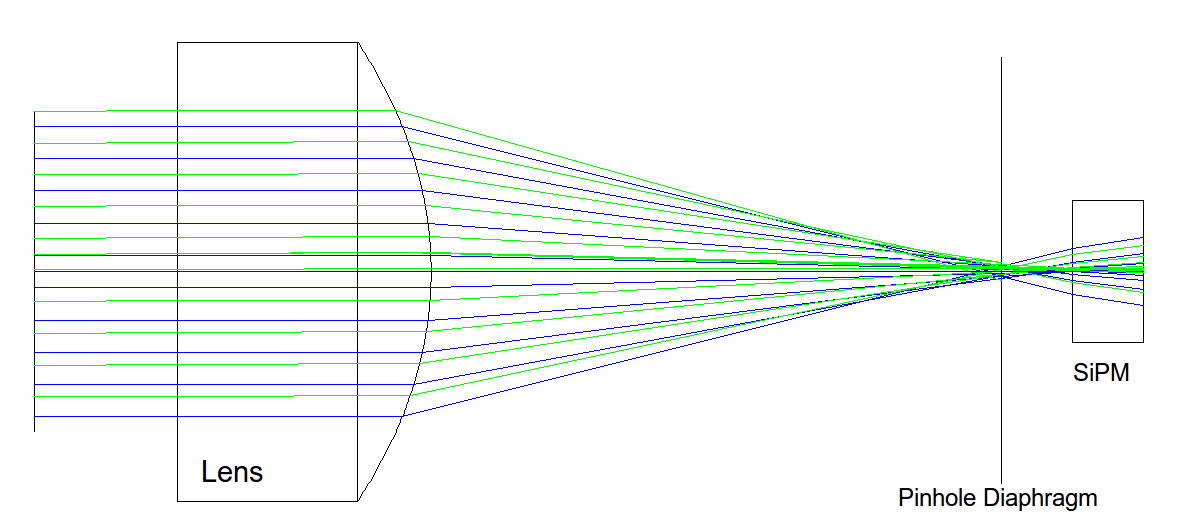
\includegraphics[width=0.7\linewidth]{sipm_zemax}
\caption{Zemax simulation of SiPM collimator.}
\label{fig:sipm_pde}
\end{figure}

Acoording to Zemax simulation, the FOV will be $2.8{^\circ}x2.8{^\circ}$,
thus we have tolerance for match both laser FoV and SiPM to cover fast axis of laser beam $(0.1{^\circ}x2.5{^\circ}$).



\subsection{Completed SiPM module}

The finished SiPM PCB is shown in the figure \ref{fig:sipm_PCB}
It consist of readout electronics for SiPM, laser driver and TDC chip, thereby integrates all functions of LiDAR itself: driving laser diode, generating high voltage for SiPM, readout and amplification of SiPM signal and measuring time delay between outgoing and return impulse.

\begin{figure}[h]
\center{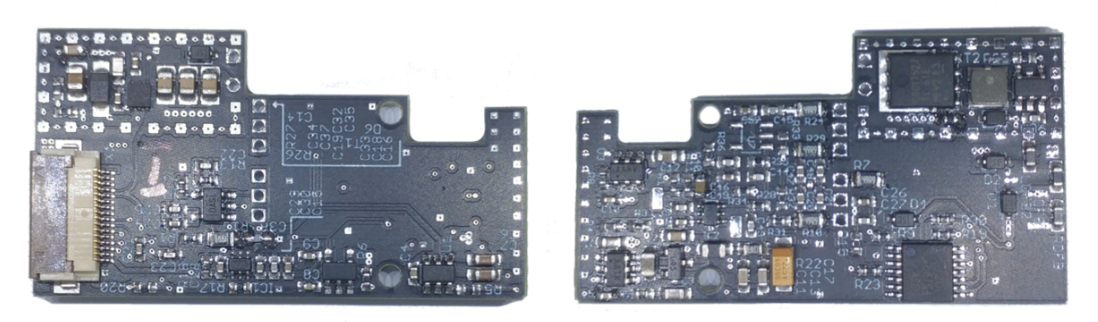
\includegraphics[width=0.85\linewidth]{sipm_PCB}} 
  \caption{Upper and lower side of SiPM PCB.}%
\label{fig:sipm_PCB} % or change caption location
\end{figure}

The assembled SiPM collimator with already attached SiPM to the bottom of tube is shown in figure \ref{fig:sipm_collimator}.
\begin{figure}[h]
\center{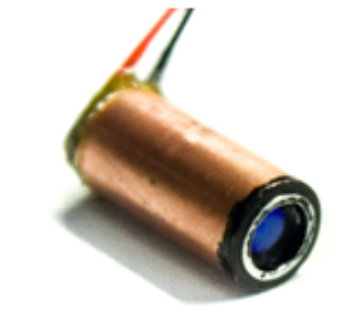
\includegraphics[width=0.3\linewidth]{sipm_collimator}} 
  \caption{Assembled SiPM collimator with integrated SiPM.}%
\label{fig:sipm_collimator} % or change caption location
\end{figure}





\section{Final implementation}

\begin{figure}[H]
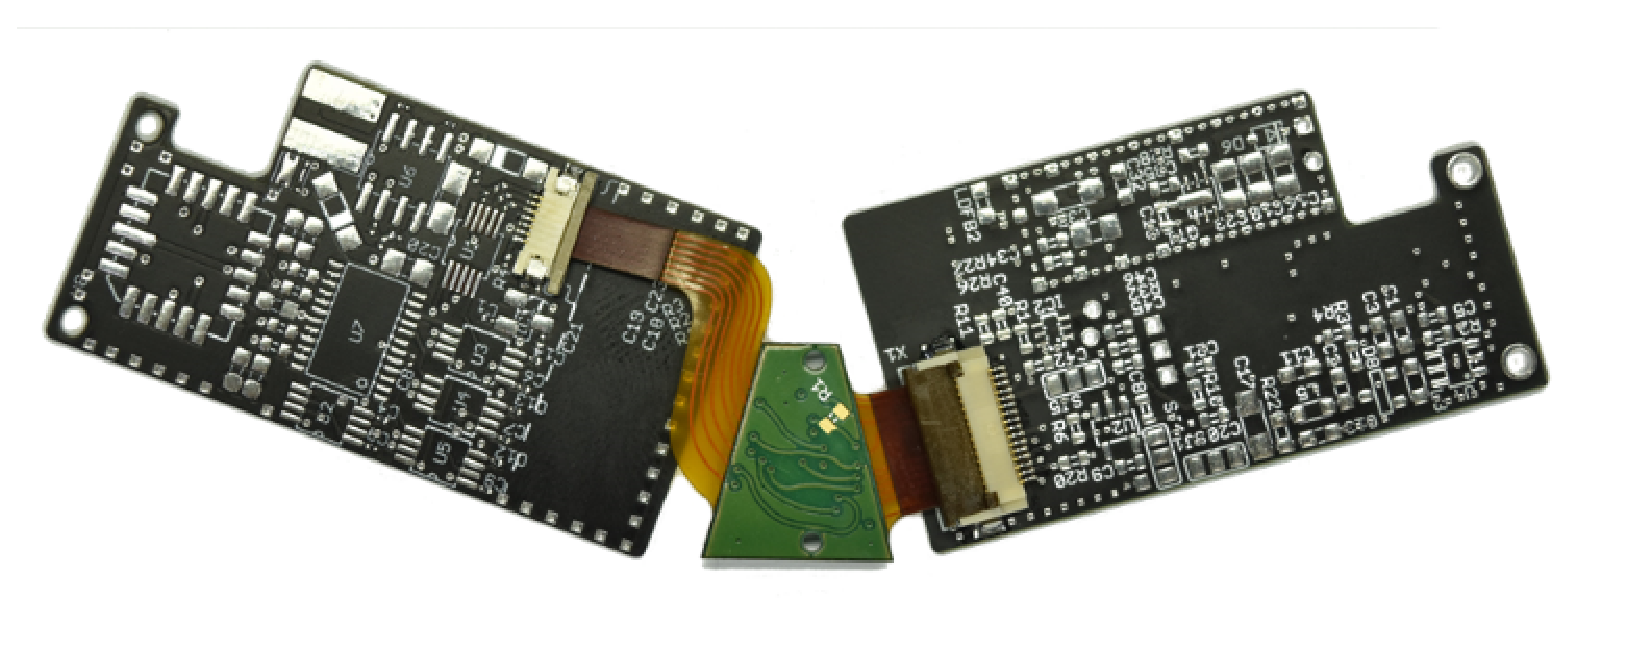
\includegraphics[width=0.75\linewidth]{flex_PCB}
\caption{Zemax simulation of SiPM collimator.}
\label{fig:sipm_pde}
\end{figure}

Picture of real submodule here
% \chapter{Hardware}
\section{Logic of submodule electronics}

All the logic of the submodule is shown in the figure \ref{fig:submodule_logic}.

\begin{figure}[H]
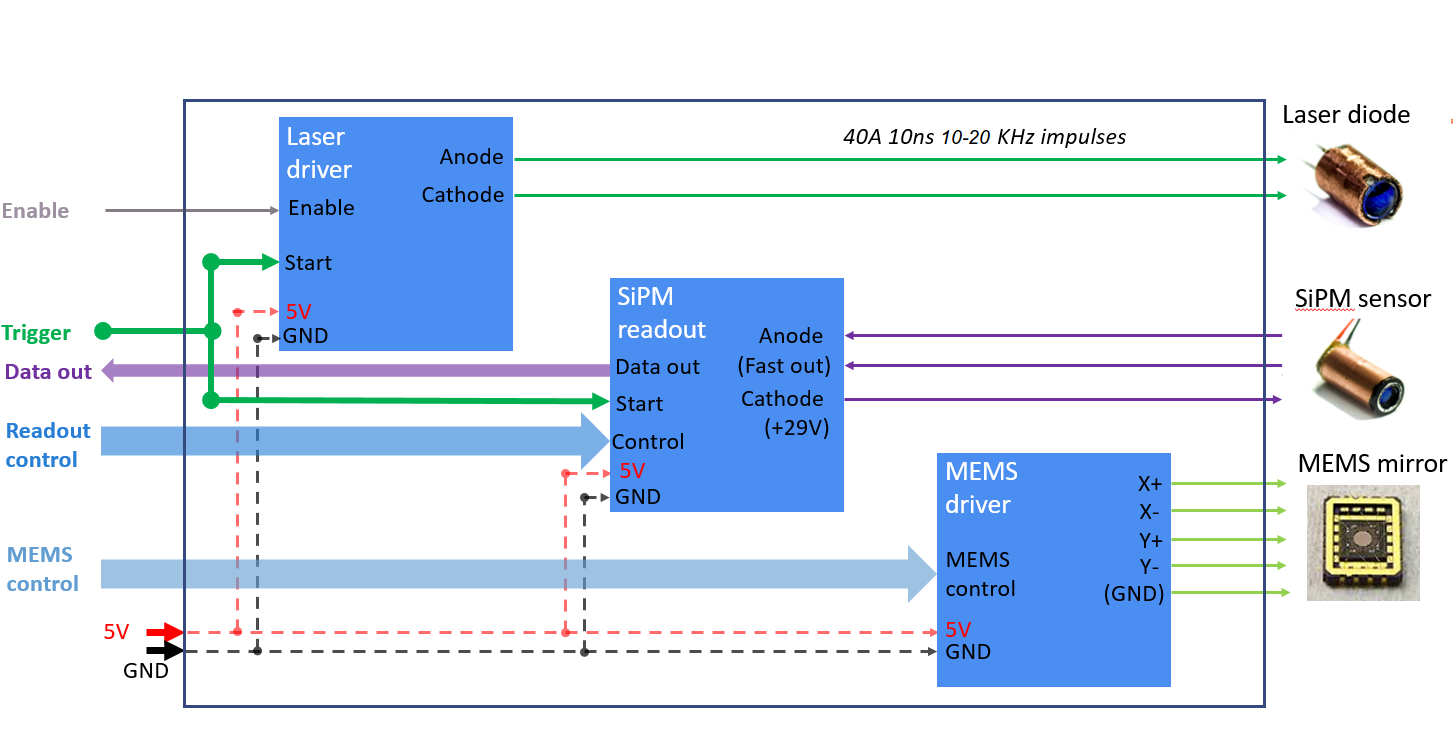
\includegraphics[width=1.05\linewidth]{logic}
\caption{Logic diagram of submodule electronics.}
\label{fig:submodule_logic}
\end{figure}

MEMS driver works independently from other modules, controlling only MEMS mirror. SiPM and Laser driver are joint by trigger signal. Laser driver utilize for shooting of laser diode, SiPM board generating high voltage for SiPM, performs readout and amplification of SiPM signal and measuring time delay between outgoing and return impulse by TDC chip.
Power supply for all components is +5V. Each components are described in detail below.

\subsection{Laser driver logic}
It is very easy to operate a laser diode, in addition to power supply (+5V) of a laser driver, we just need provide LH (Logical High, 3.3V for here) to the Enable input and clock signal with desirable frequency $f$ to the Trigger input, after that Laser driver repeats electrical 40A pulses with 10ns width for Laser diode.

\begin{figure}[H]
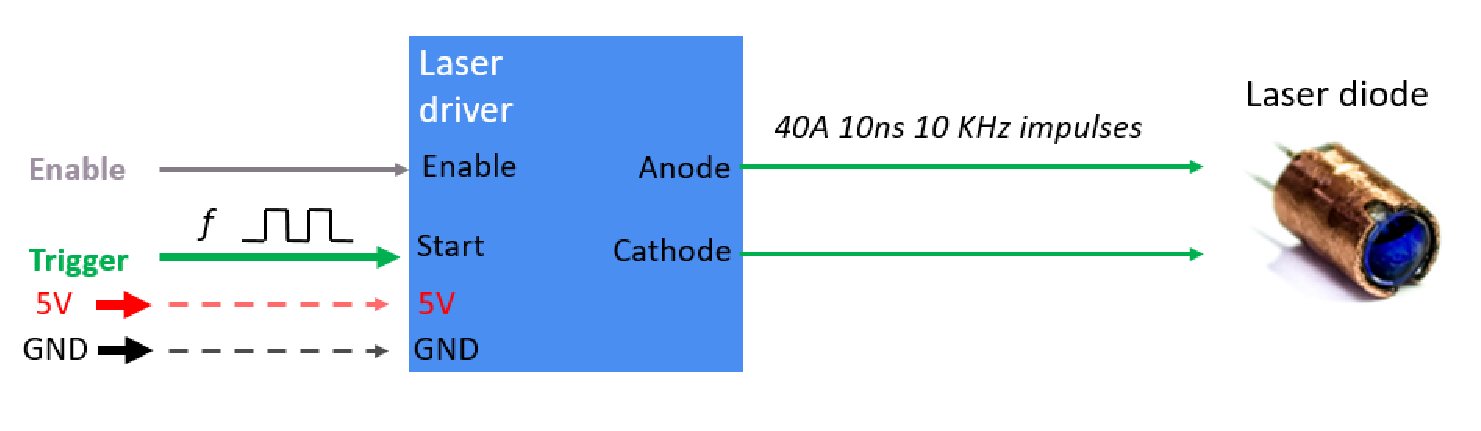
\includegraphics[width=1\linewidth]{ld_logic}
\caption{Logic diagram of laser driver.}
\label{fig:real_submodule}
\end{figure}

\subsection{MEMS driver logic}

MEMS driver board has a power (+5V) and control (SPI) input which are used for the control of MEMS mirror via SPI commands to 16-bit DAC, which produces a high-voltage (160V) 4-channel signal (X+, X-, Y+, Y-). 
We used 16-bit DAC with 20MHz SPI speed. 
Filter clocks input is used for set LPF cutoff frequency, to avoid high frequency which can induce resonance and damage of the mirror.


\begin{figure}[H]
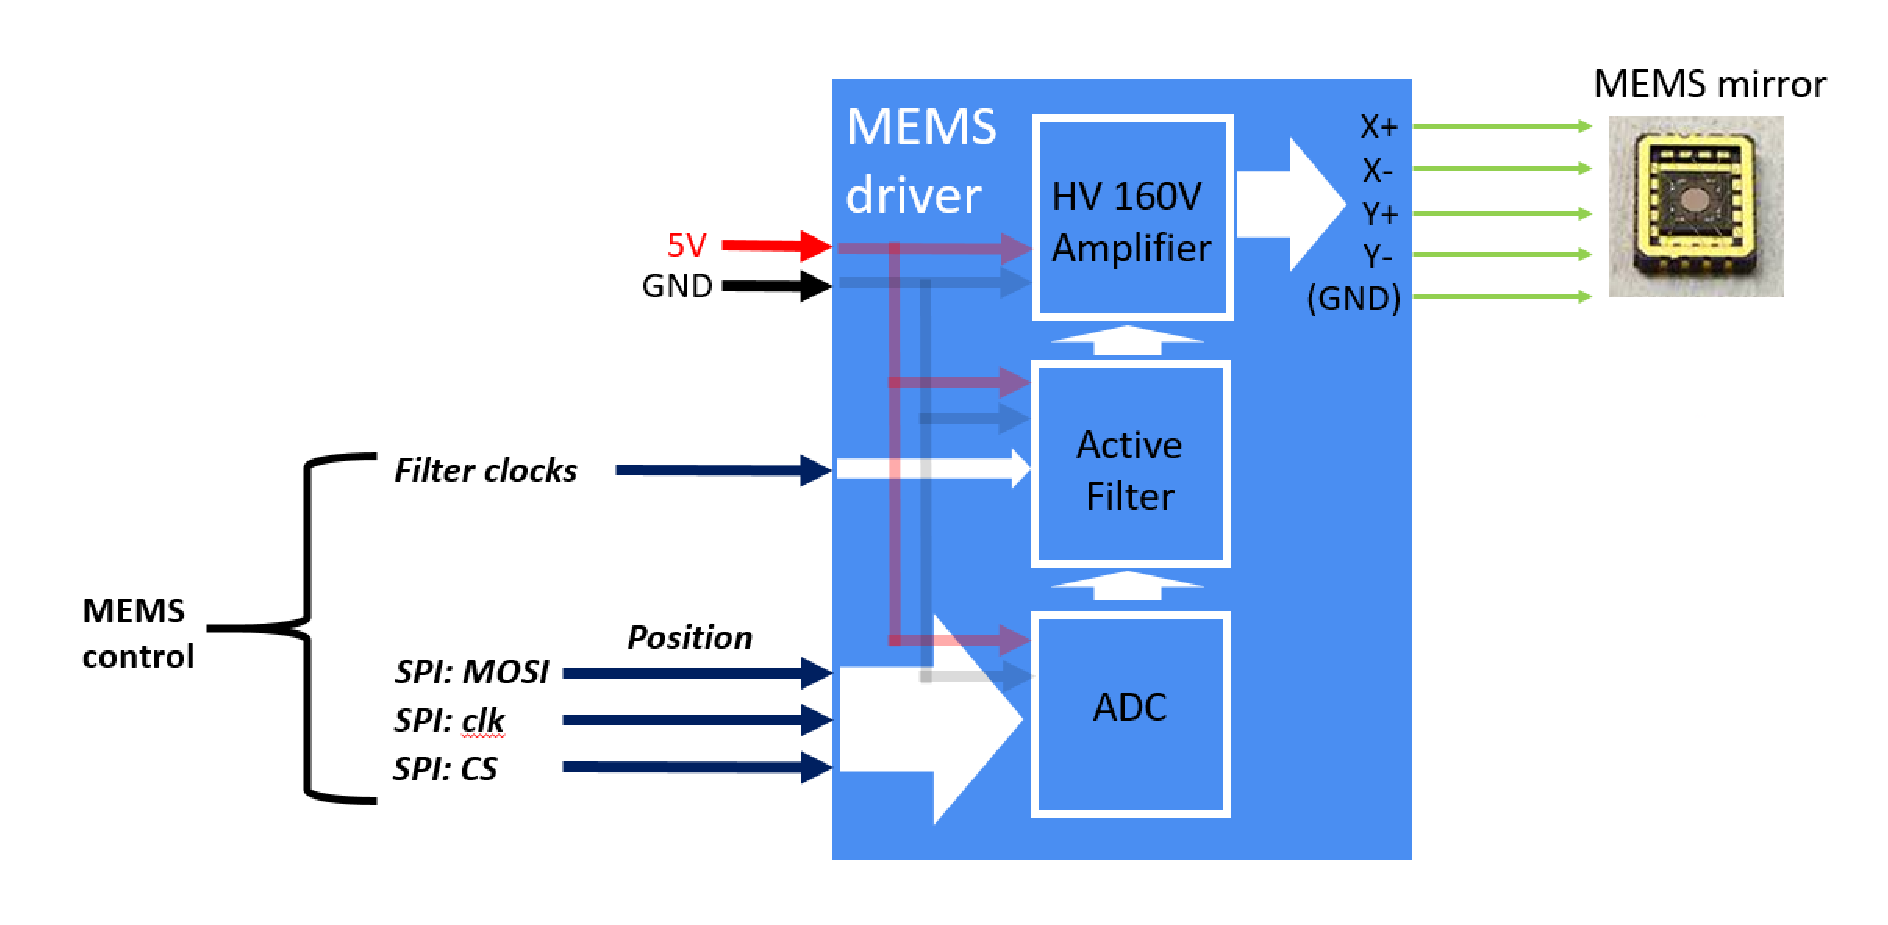
\includegraphics[width=1\linewidth]{mems_logic}
\caption{Logic diagram of MEMS driver.}
\label{fig:real_submodule}
\end{figure}


To form a trajectory with maximum possible FPS, for axis X applied voltage sine and for axis Y applied voltage like pulse with triangle shape. Depending on sine frequency we can get different number of lines, that makes vertical resolution very flexible as shiown in figure \ref{fig:mems_real_trajectories}.



\begin{figure}[H]
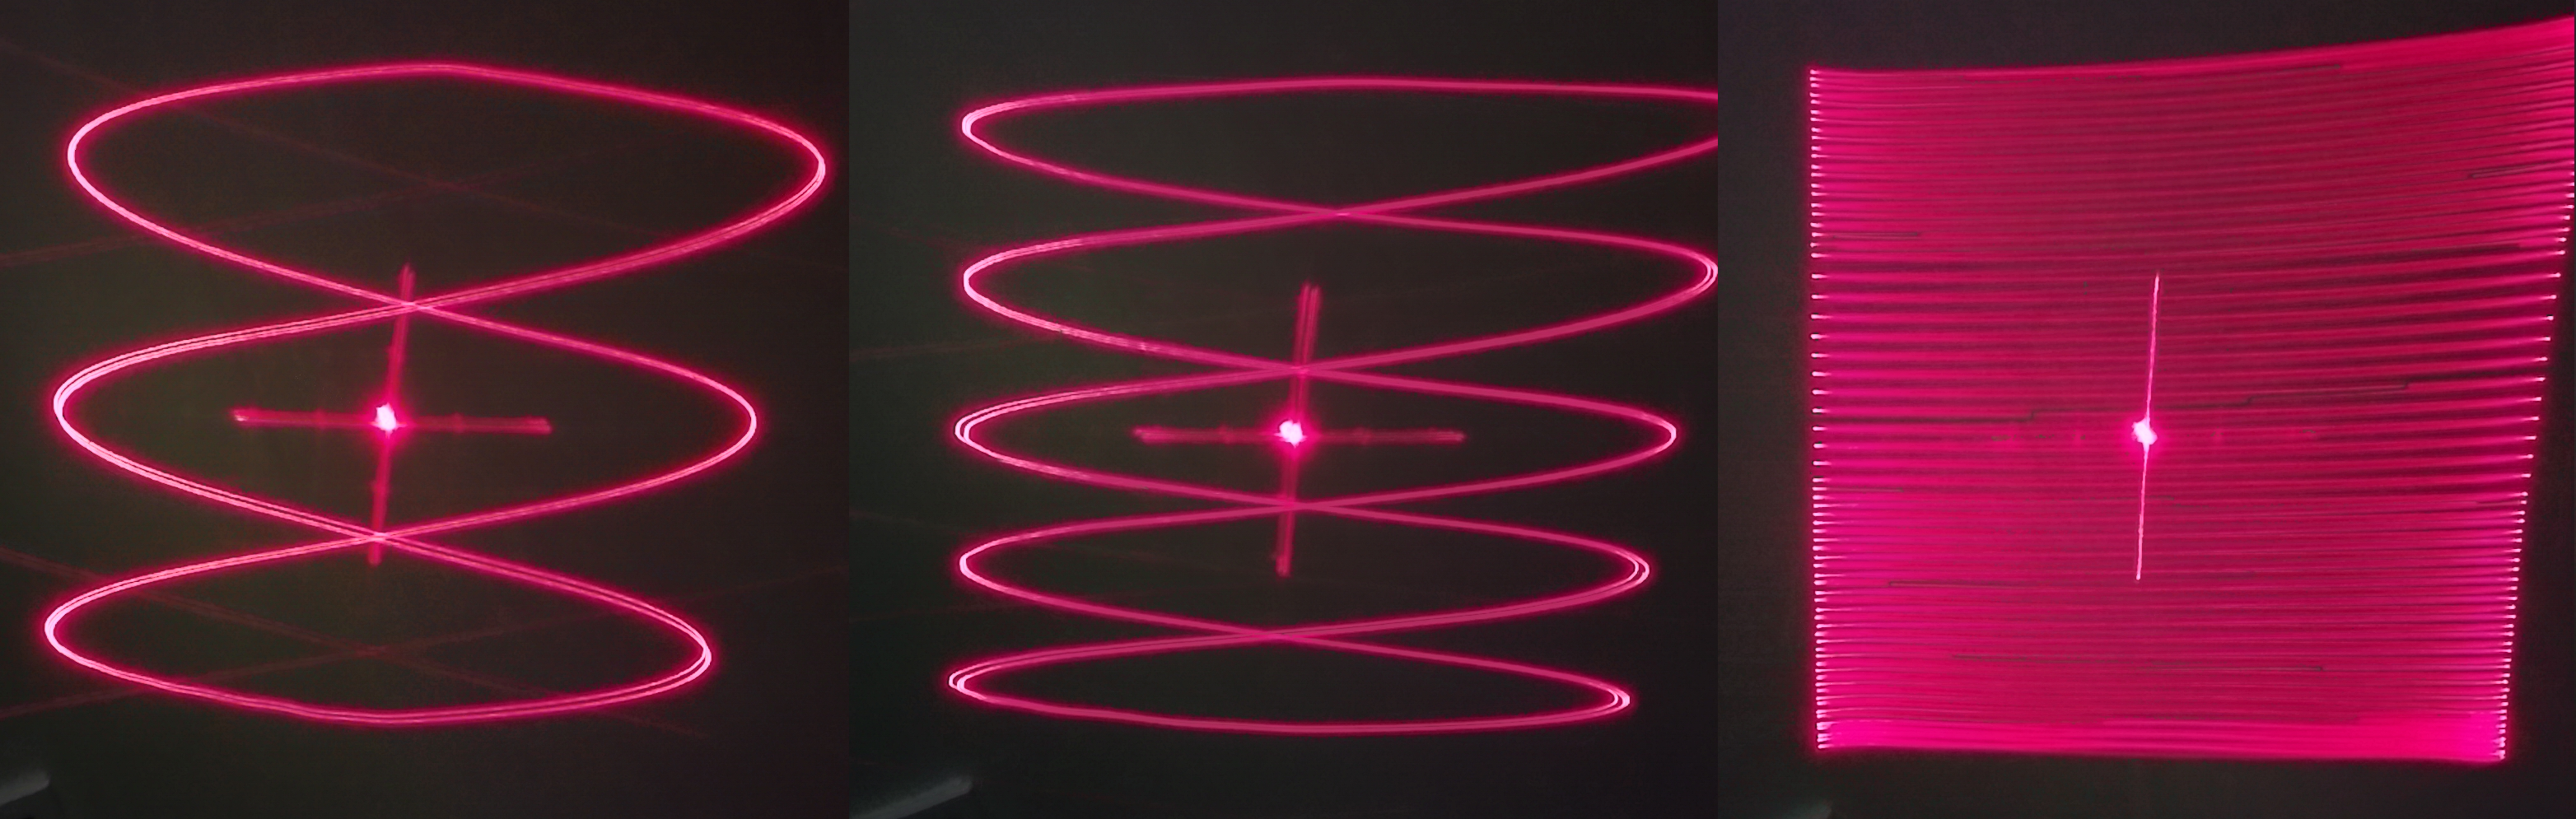
\includegraphics[width=1\linewidth]{mems_real_trajectories}
\caption{Photo of different resolutions: 4,8 and 60 lines.}
\label{fig:mems_real_trajectories}
\end{figure}





\subsection{SiPM logic}

SiPM board has a power (+5V) which is transformed to +29V for SiPM bias voltage and $\pm5 V$ for amplifier voltage. Readout contol (SPI) input are used for the control of TDC.
After aplification of the SiPM output (Fast out), signal goes to comparator, if level exceeds treshold, LH is provided to TDC Stop input.
After that, when TDC finished time calculation, Interrupt pin is fired and the result can be read by SPI DOUT.
Ref clk input is waiting for high frequecy clock signal - 12.5 MHz in our case, which is used for TDC measurement.



\begin{figure}[H]
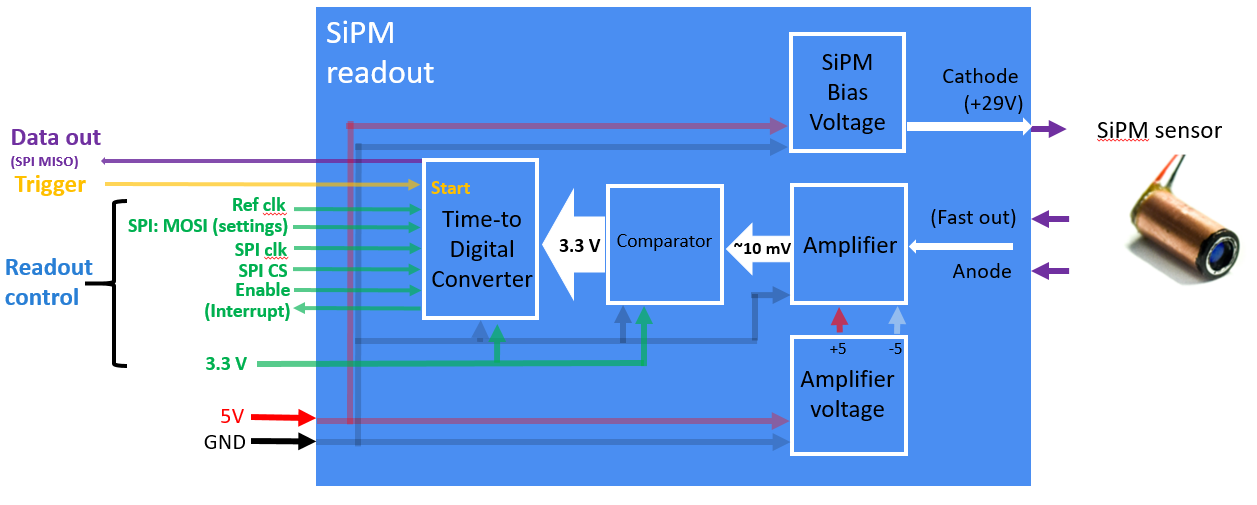
\includegraphics[width=1\linewidth]{sipm_logic}
\caption{Designed and real assembled submodule.}
\label{fig:real_submodule}
\end{figure}


During descring green board also desribe power board

\section{Control board}
In the beginning, logic control was performed by the micro CPU, which allowed to quickly develop a pilot version of the control board. Then, with growing needs, it became obvious the need to use FPGA, giving advantages in speed and parallelism, so the final version of the control board was completely implemented on FPGA.

The clock was modified via PLL from 50 to 64 MHz.
FPGA has faster clock + allow parallel \& less jitter.

\begin{figure}[H]
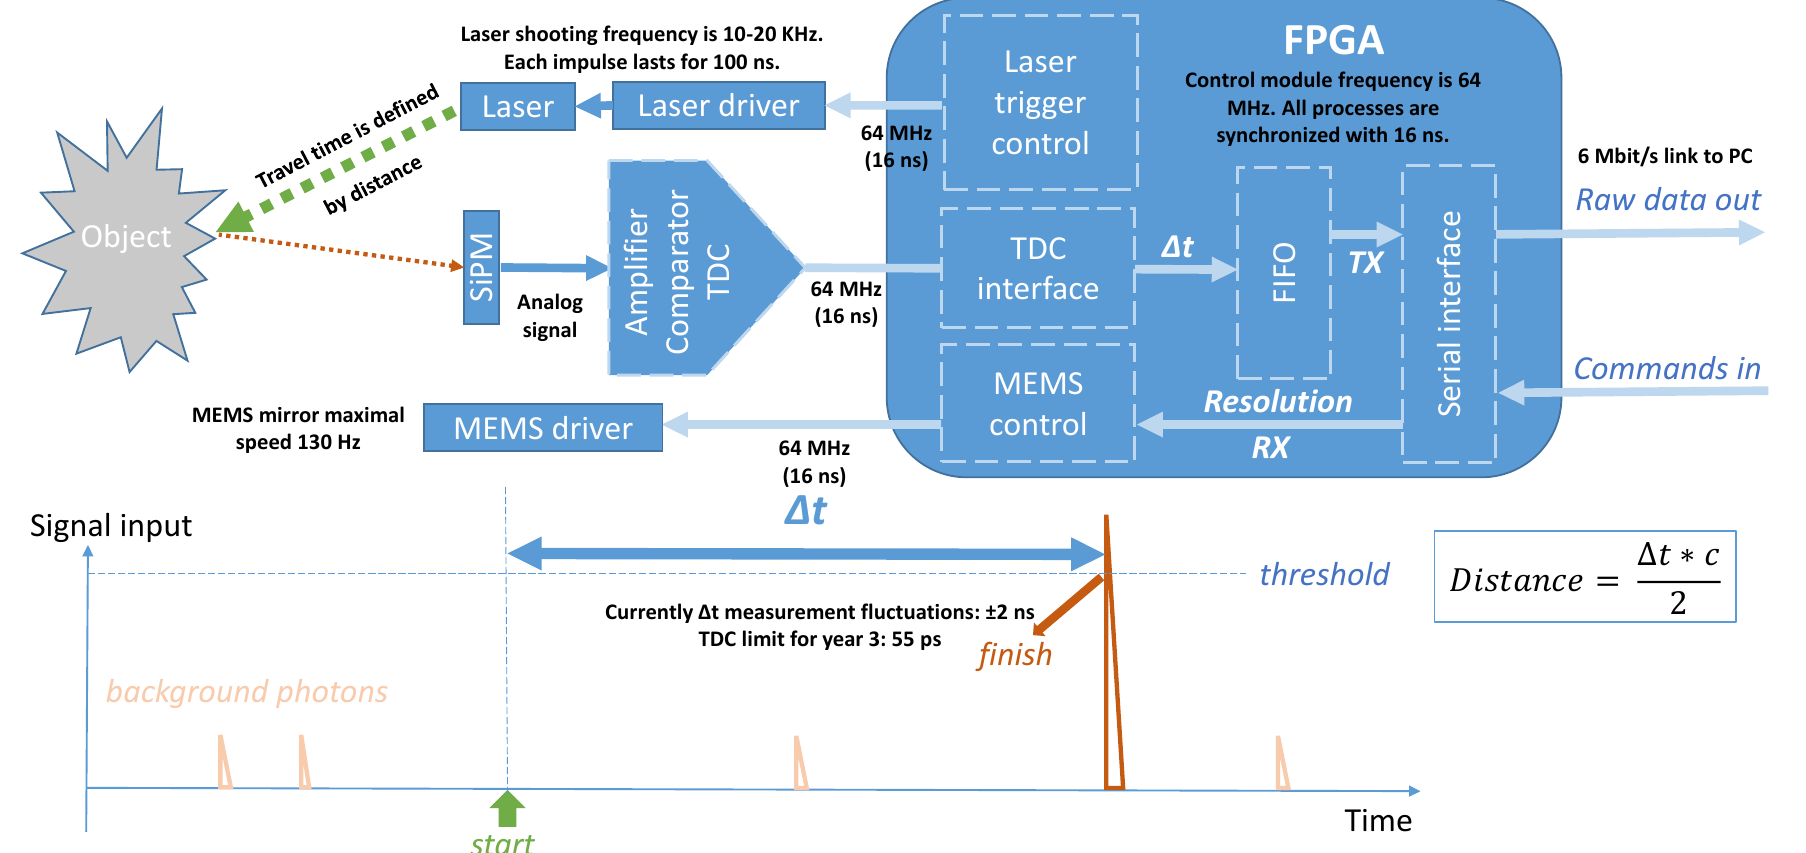
\includegraphics[width=1.1\linewidth]{control}
\caption{Designed and real assembled submodule.}
\label{fig:real_submodule}
\end{figure}



AZAZAZA
Their long-term aid ~\cite{Haggarty:01} ~\cite{Haggarty:02}

The \Gls{latex} typesetting markup language is specially suitable 
for documents that include \gls{maths}. \Glspl{formula} are 
rendered properly an easily once one gets used to the commands.
 
Given a set of numbers, there are elementary methods to compute 
its \acrlong{gcd}, which is abbreviated \acrshort{gcd}. This 
process is similar to that used for the \acrfull{lcm}.

\renewcommand{\bibname}{References}
\bibliographystyle{unsrt}
\bibliography{refs}

% \chapter{Appedix A} % to remove number we use * + this one is needed in the biblio \addcontentsline{toc}{chapter}{Appendix A} 
% \section{azazaz}
% \paragraph{aza}
% % \label{my_desire}
% Hello to everyone, I really want to make
% Latex diploma and I will
% \subsection{sub}
% this is sub..

% \section{azazaz}
% asdasd as I said in ~\ref{my_desire}

% asd
% s

% \begin{enumerate}
% \item xczxc
% \item xdf
% \item fdgf
% \end{enumerate}

% \begin{itemize}
% \item dfdf
% \item sdfs
% \item sdfs
% \end{itemize}

% \section*{azazaz}

\begin{appendices}
  \chapter{Consectetur adipiscing elit}
  \section{First part}
  asxdsdsa
  \section{Second}
  I'm a second part!
  \chapter{Mauris euismod}
  ~\ref{fig:skku}
\end{appendices}
% это титульный лист



\end{document}


